\documentclass[10pt]{beamer}%
\usetheme[progressbar = foot]{metropolis} 
\usecolortheme[cautious]{owl} %owl-defined colours will be available as OwlRed, OwlGreen, and so forth.
\setbeamercolor{title separator}{fg=OwlGreen}

% input

\usepackage[utf8]{inputenc}%
\usepackage{lmodern} %Type1-font for non-english texts and characters
\usepackage[USenglish]{babel} %francais, polish, spanish, ...
\usepackage[T1]{fontenc}

\usepackage{ragged2e}%for text justification by default
\justifying

% graphics
%% Figures %%%%%%%%%%%%%%%%%%%%%%%%%%%%%%%%%%%%%%%%%%%%%%%%%%
\usepackage{graphicx}
\usepackage{xcolor}%for color mixing
\definecolor{mypurple}{rgb}{0.231, 0.204, 0.471}
\definecolor{mypurple1}{rgb}{0.573, 0.467, 0.675}
\definecolor{mypurple2}{rgb}{0.122, 0.016, 0.224}

\definecolor{mygreen}{rgb}{0.153, 0.443, 0.365}
\definecolor{myorange}{rgb}{0.882, 0.612, 0.224}

\definecolor{bostonuniversityred}{rgb}{0.8, 0.0, 0.0}
\definecolor{blendedblue}{rgb}{0.137,0.466,0.741}

\definecolor{darkred}{rgb}{0.545,0,0}

 
\usepackage{tikz} % for arrows and figures
\usetikzlibrary{positioning,decorations.pathreplacing,shapes,trees,calc}

\usepackage{amsmath}%
\usepackage{amsfonts}%
\usepackage{amssymb}%
\usepackage{graphicx}


\usepackage{booktabs}


\usepackage{hyperref}
\setlength{\arraycolsep}{3pt}

%%%%%%%%%%%%%%%%%%%%%%%%%%%%%%%%%%%%%%%%%%%%%%
%%%%%%%%%%%%%%%%% Doc info %%%%%%%%%%%%%%%%%%%
\title[\textbf{Adaptation against apparent selection}]{\textbf{Individual-level causes and population-level consequences of variation in fitness in an Alpine rodent}}
%\titlegraphic{\fcolorbox{blendedblue}{blendedblue}{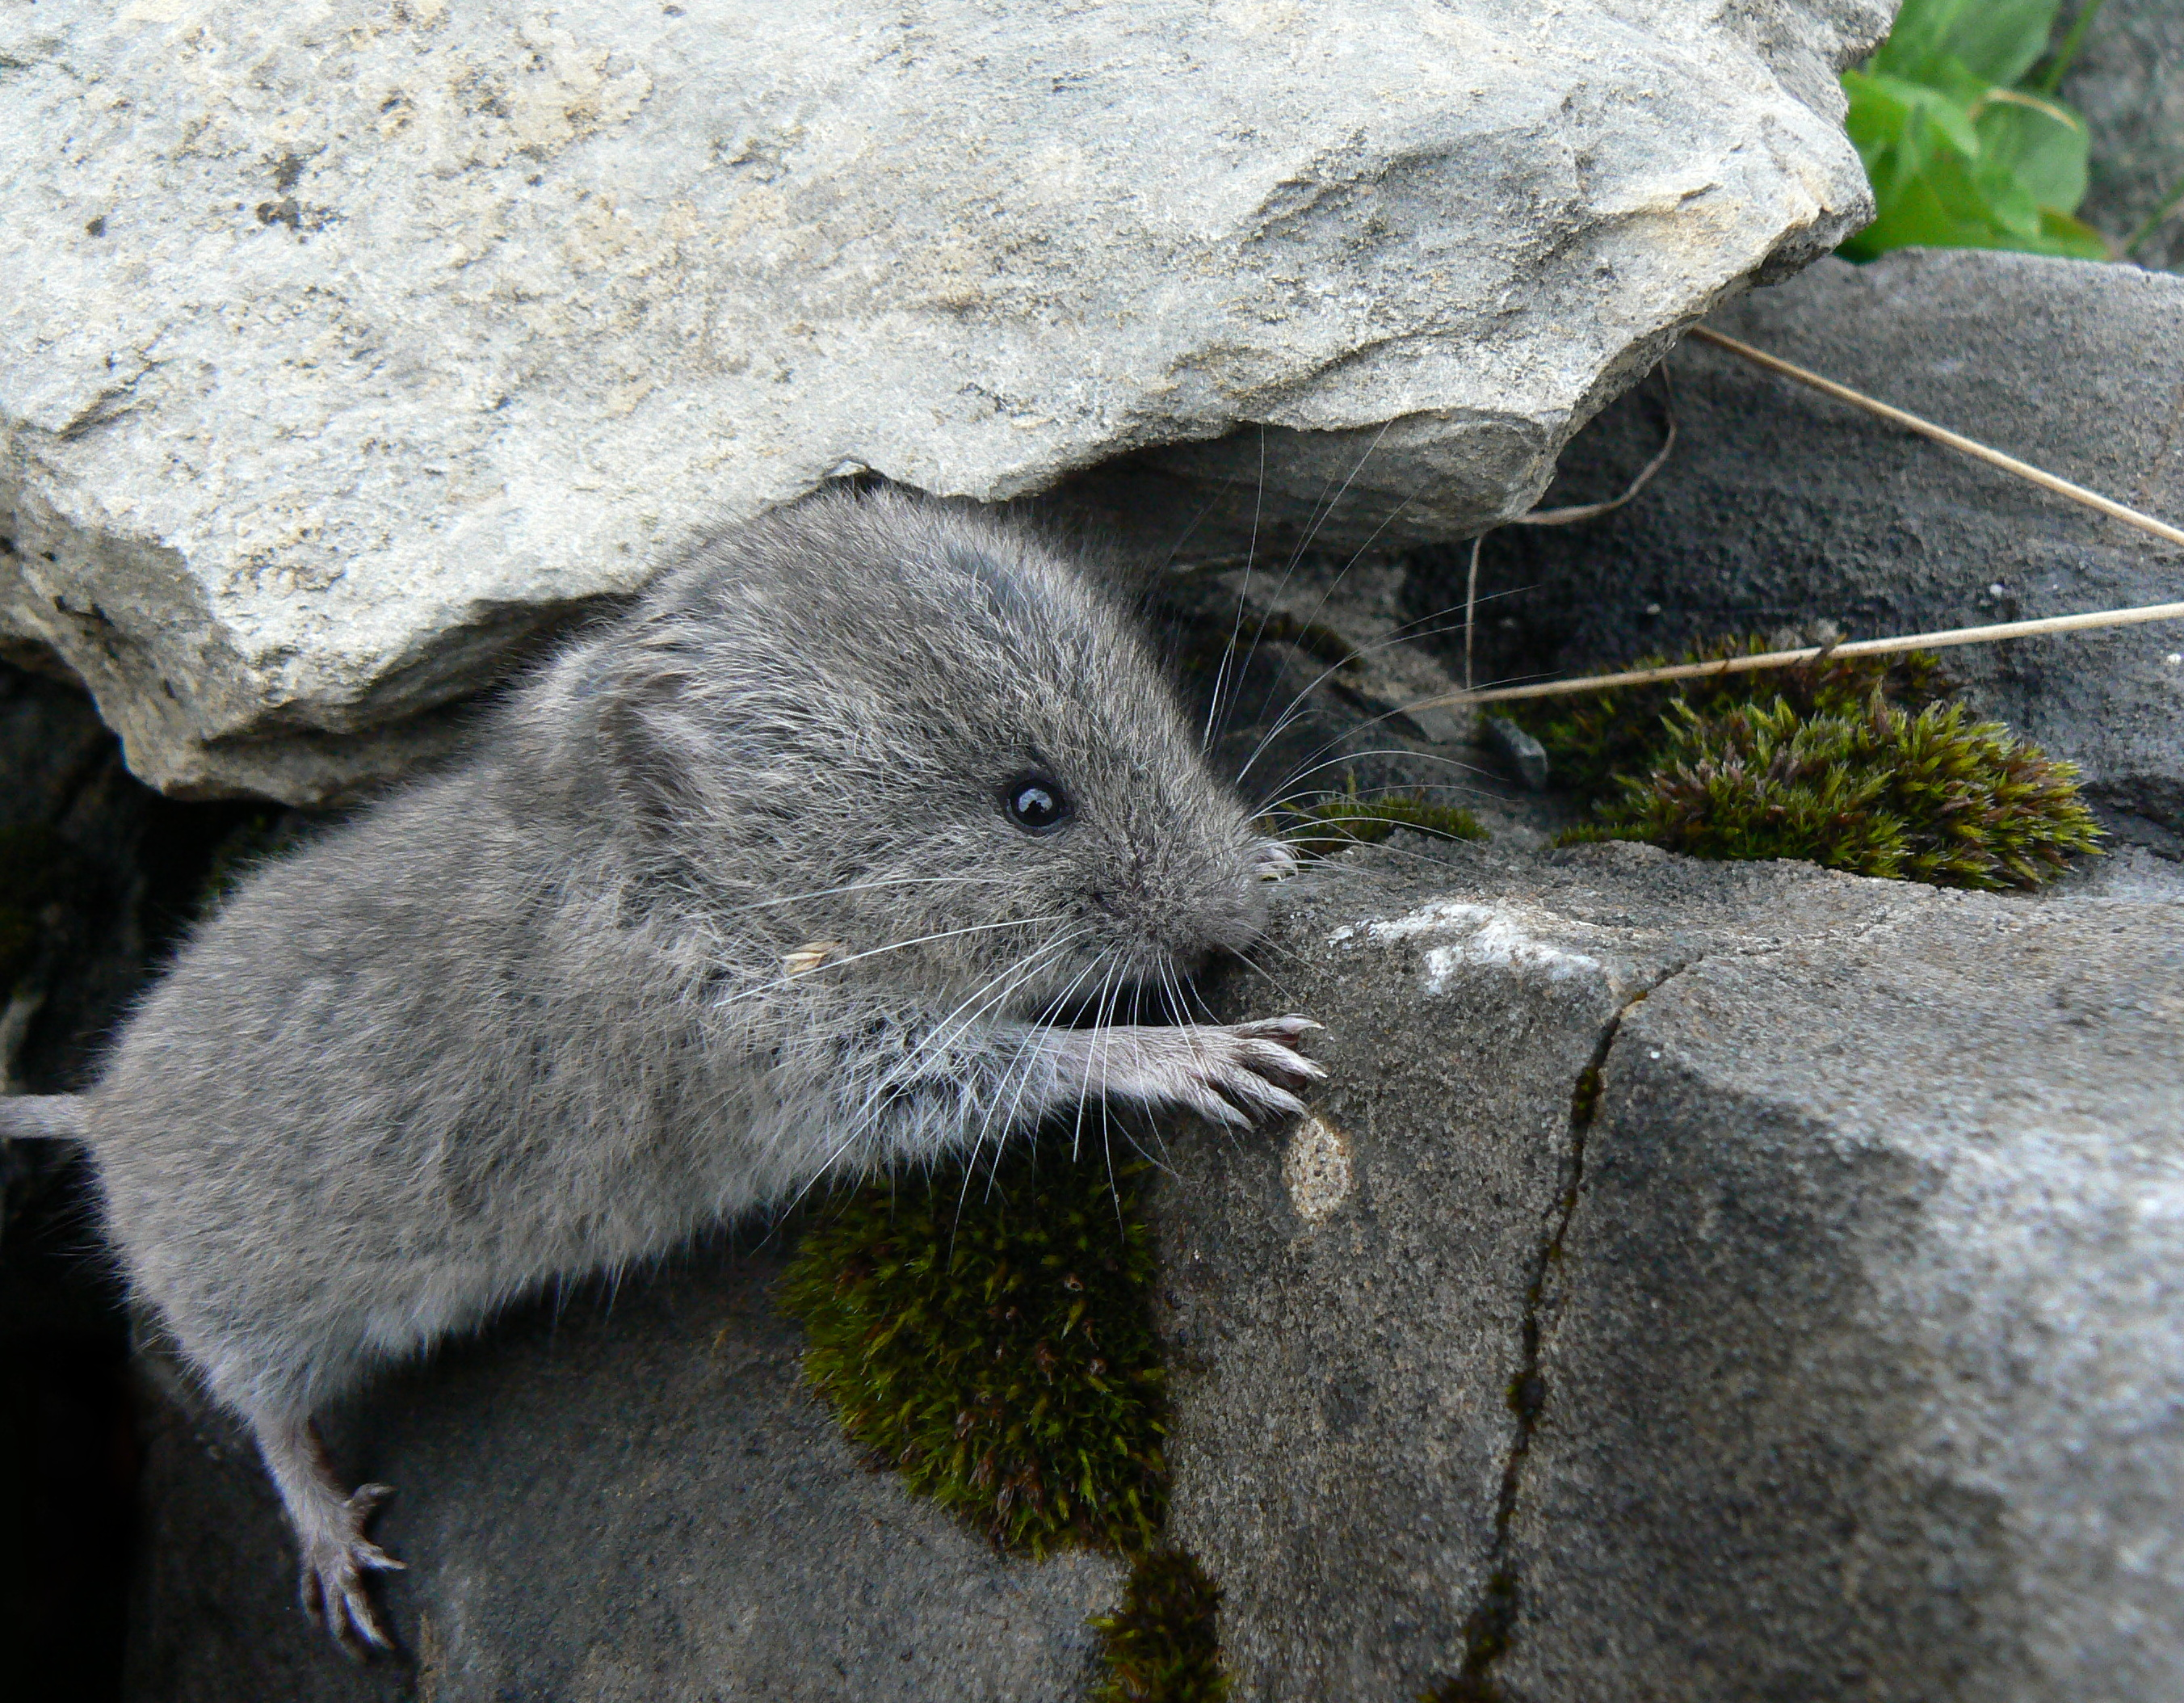
\includegraphics[width=0.45\textwidth]{Figures/cutevole}}}
%\subtitle{UOBU}
\author[\textbf{\fontfamily{pcr}\selectfont timothee.bonnet@ieu.uzh.ch}]{\textbf{Timoth\'{e}e Bonnet}}
%\date{\fcolorbox{blendedblue}{blendedblue}{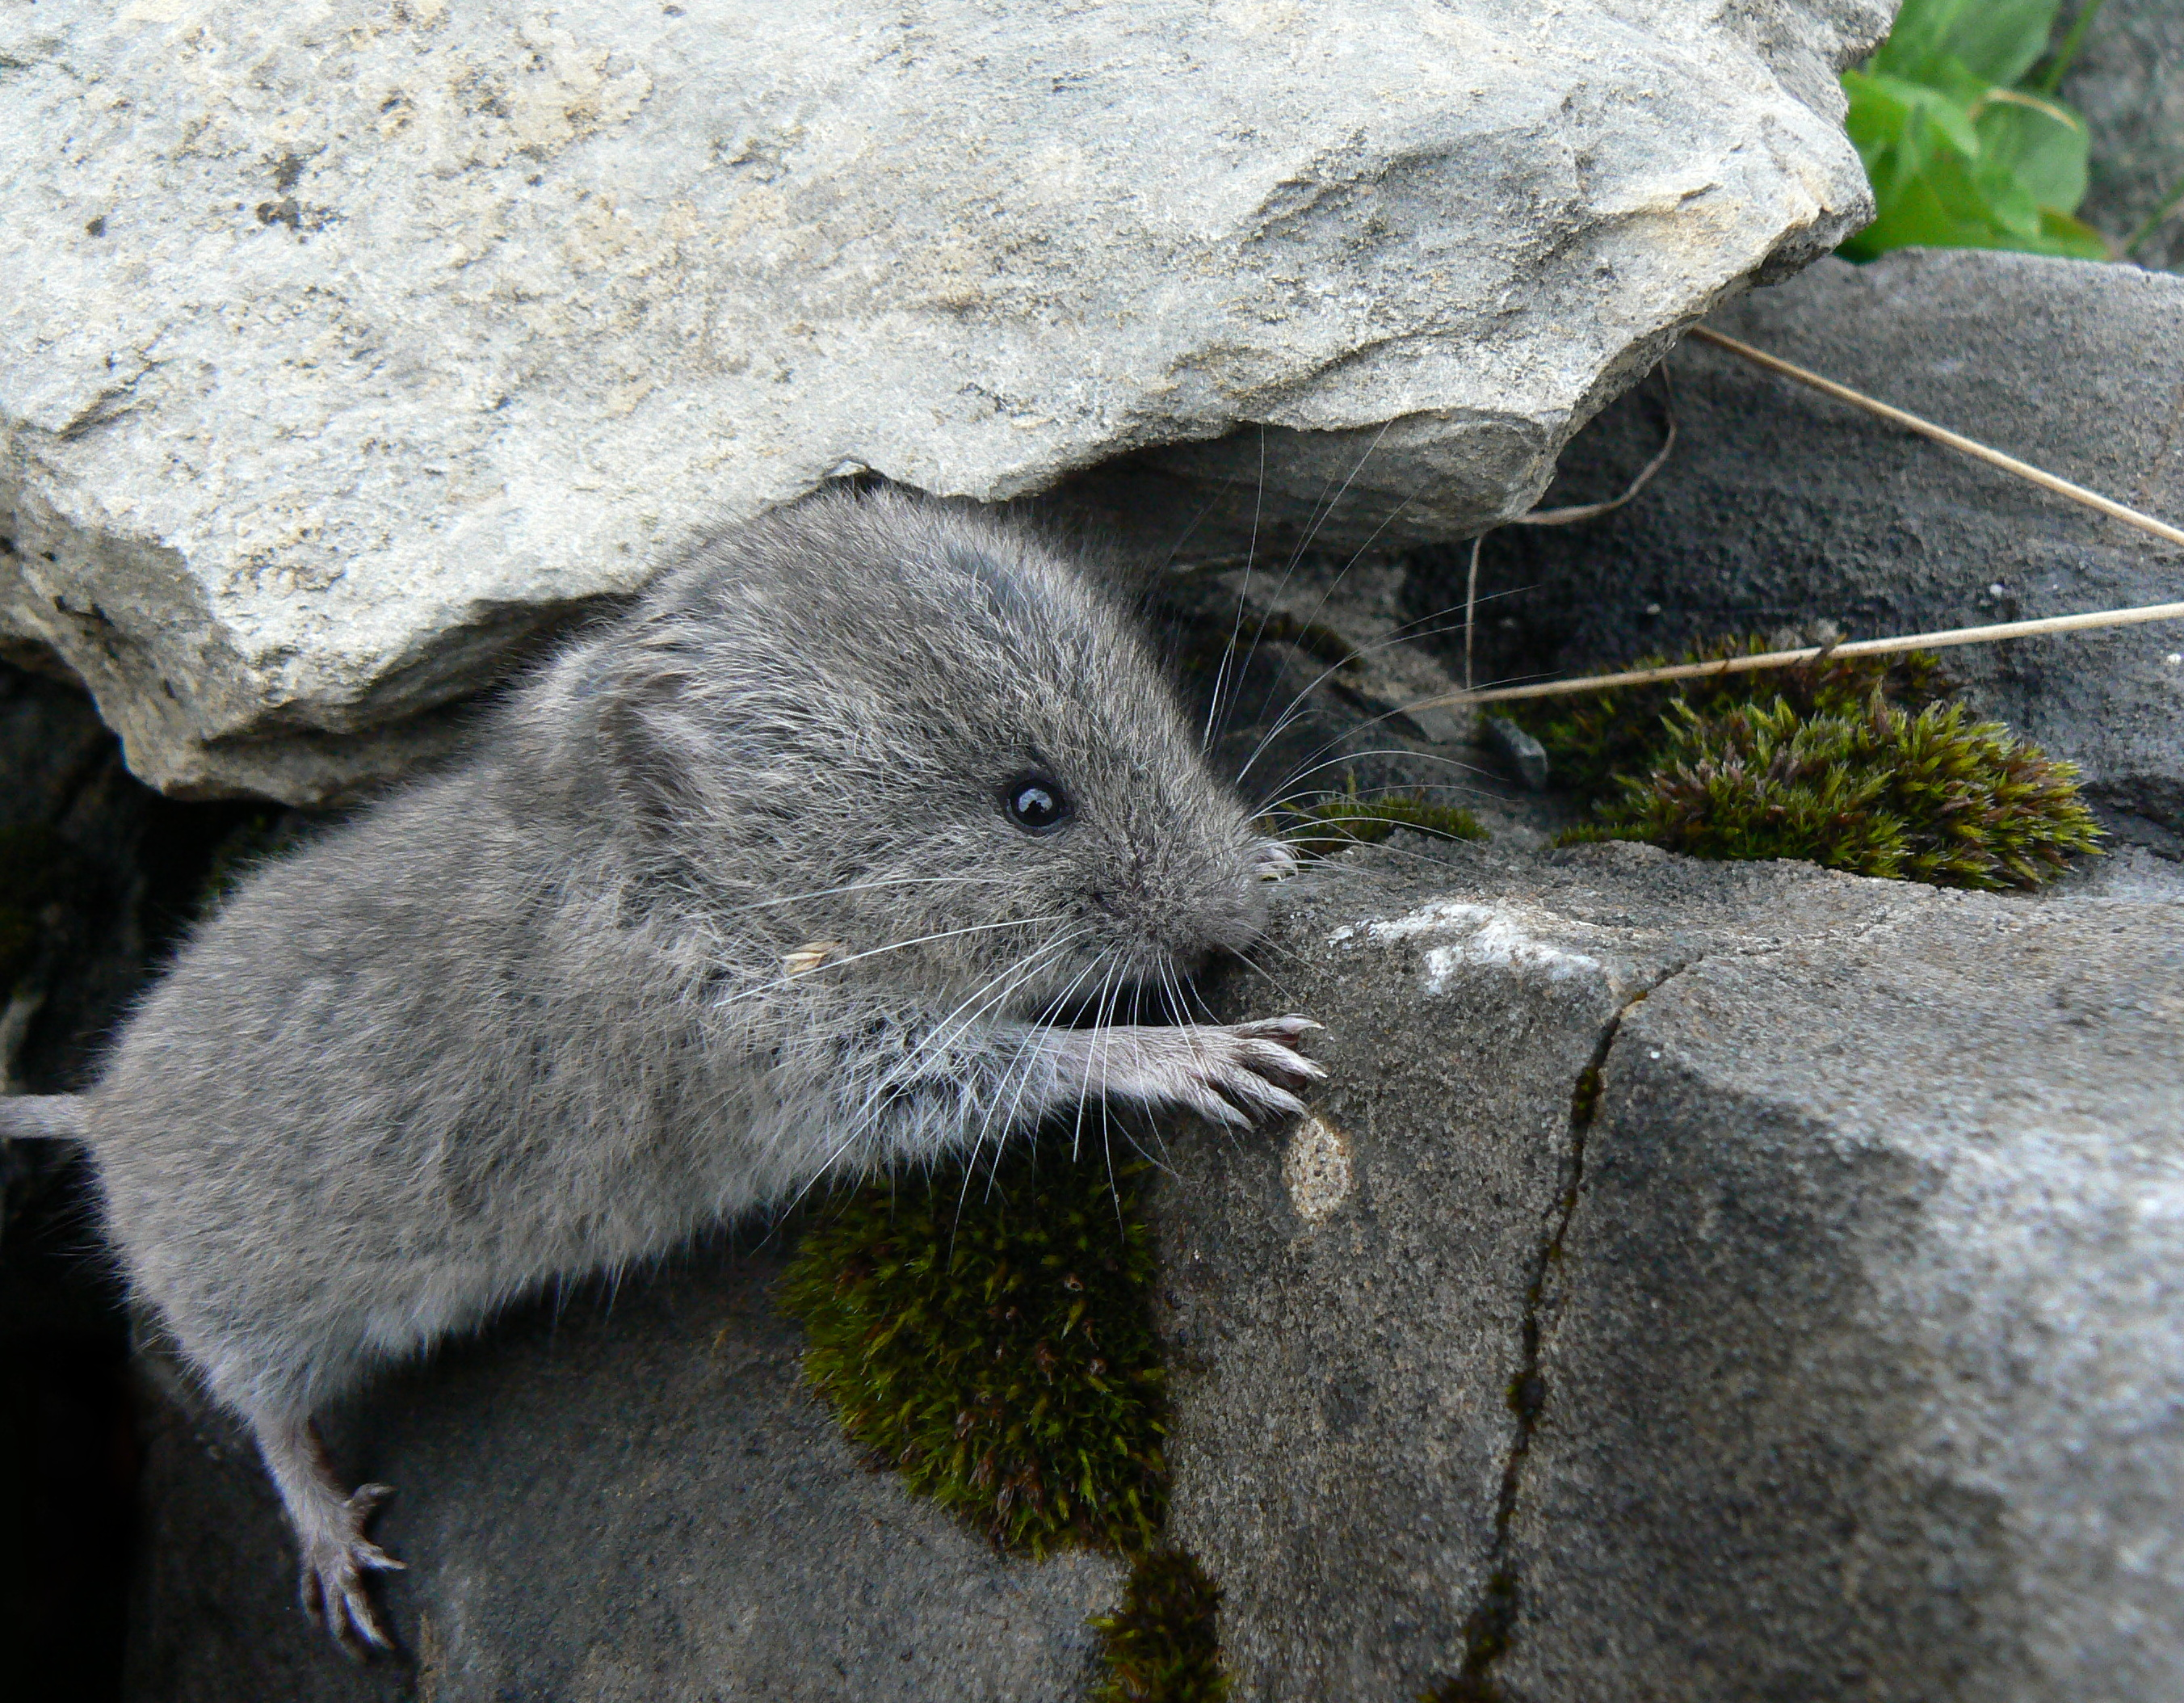
\includegraphics[width=0.35\textwidth]{Figures/cutevole}}}
\date{\vspace{1cm}}
\institute[IEU, University of Zurich]{\small Department of evolutionary biology and environmental studies (IEU) \\ \vspace{-0.1cm} \\ 
\includegraphics[width=0.3\textwidth]{Figures/uzhlogo}}



%%%%%%%%%%%%%%%%%%%%%%%%%%%%%%%%%%%%%%%%%%%%%%
\begin{document}

\begin{frame}[plain]
\maketitle
\end{frame}
%%%%%%%%%%%

%\section{Acknowledgements}

\begin{frame}[plain]

\begin{columns}
	\begin{column}[c]{0.35\textwidth}
		\begin{itemize}
		\setlength\itemsep{0.05cm}
		\small
			\item<2-> Erik Postma
		%committee
			\item<3-> Lukas Keller
			\item<3-> Barbara Tschirren
			\item<3-> Arpat Ozgul
			\item<3-> Marc Kéry 
			\item<3-> Jarrod Hadfield
		%colleagues
			\item<4-> Glauco Camenisch
			\item<5-> Ursina Tobler
			\item<6-> Dominique Waldvogel
			\item<6-> Martina Schenkel
			\item<6-> Vicente Garc{\'{i}}a-Navas
			\item<7-> Andres Hagmayer
			\item<8-> Koen van Benthem
			\item<8-> Marjolein Bruijning
			\item<8-> Eelke Jongejans	
			\item<9-> Pirmin Nietlisbach
			\item<9-> Philipp Becker
			\item<9-> Judith Bachmann
					
%former colleagues?

%friends and family
		\end{itemize}
	\end{column}
	\begin{column}[c]{0.7\textwidth}
		%Residual
		\begin{figure}[c]
			\begin{tikzpicture}
				\uncover<2->{\node (erik) at (0,0) {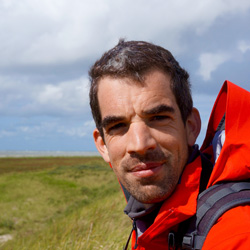
\includegraphics[width = 0.2 \textwidth]{Figures/Erik}};}
				\uncover<3->{\node (lukas) at ($(erik)+(1.2,0)$) {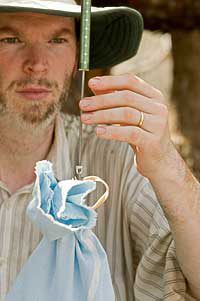
\includegraphics[width = 0.15 \textwidth]{Figures/Lukas}};
				\node (barbara) at ($(lukas)+(1,0)$) {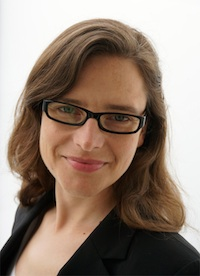
\includegraphics[width = 0.15 \textwidth]{Figures/Barbara}};
				\node (arpat) at ($(barbara)+(1.3,0)$) {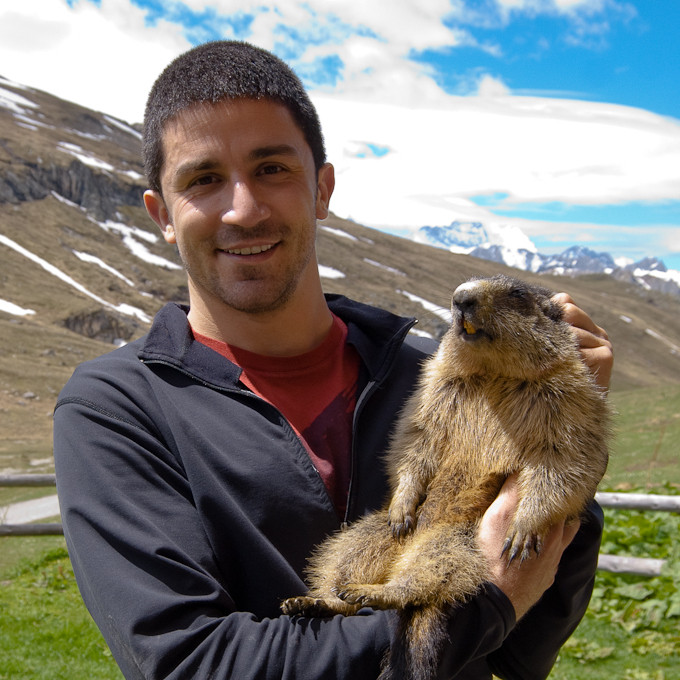
\includegraphics[width = 0.2 \textwidth]{Figures/Arpat}};
				\node (marc) at ($(arpat)+(1.2,0)$) {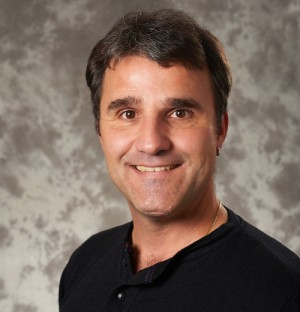
\includegraphics[width = 0.2 \textwidth]{Figures/Marc}};
				\node (jarrod) at ($(marc)+(1.3,0)$) {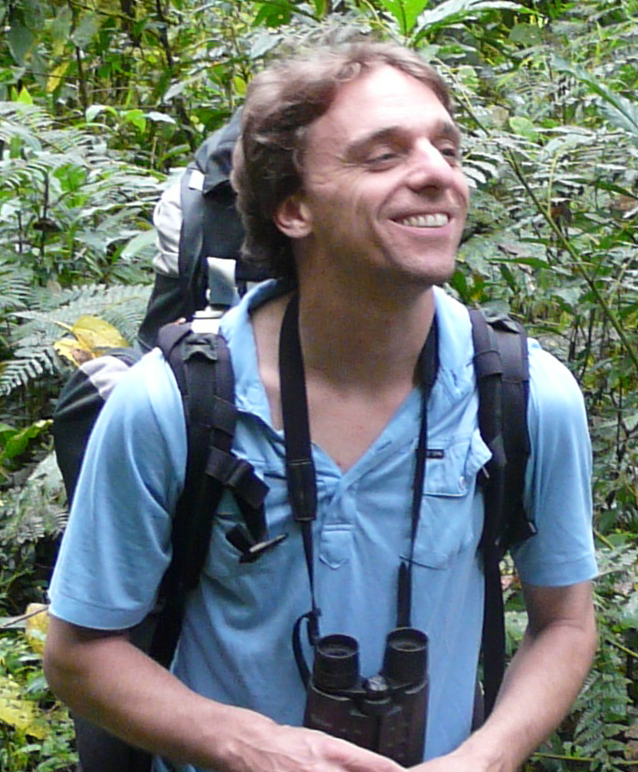
\includegraphics[width = 0.2\textwidth]{Figures/Jarrod}};}
				\uncover<4->{\node (glauco) at ($(erik)+(0,-1.4)$) {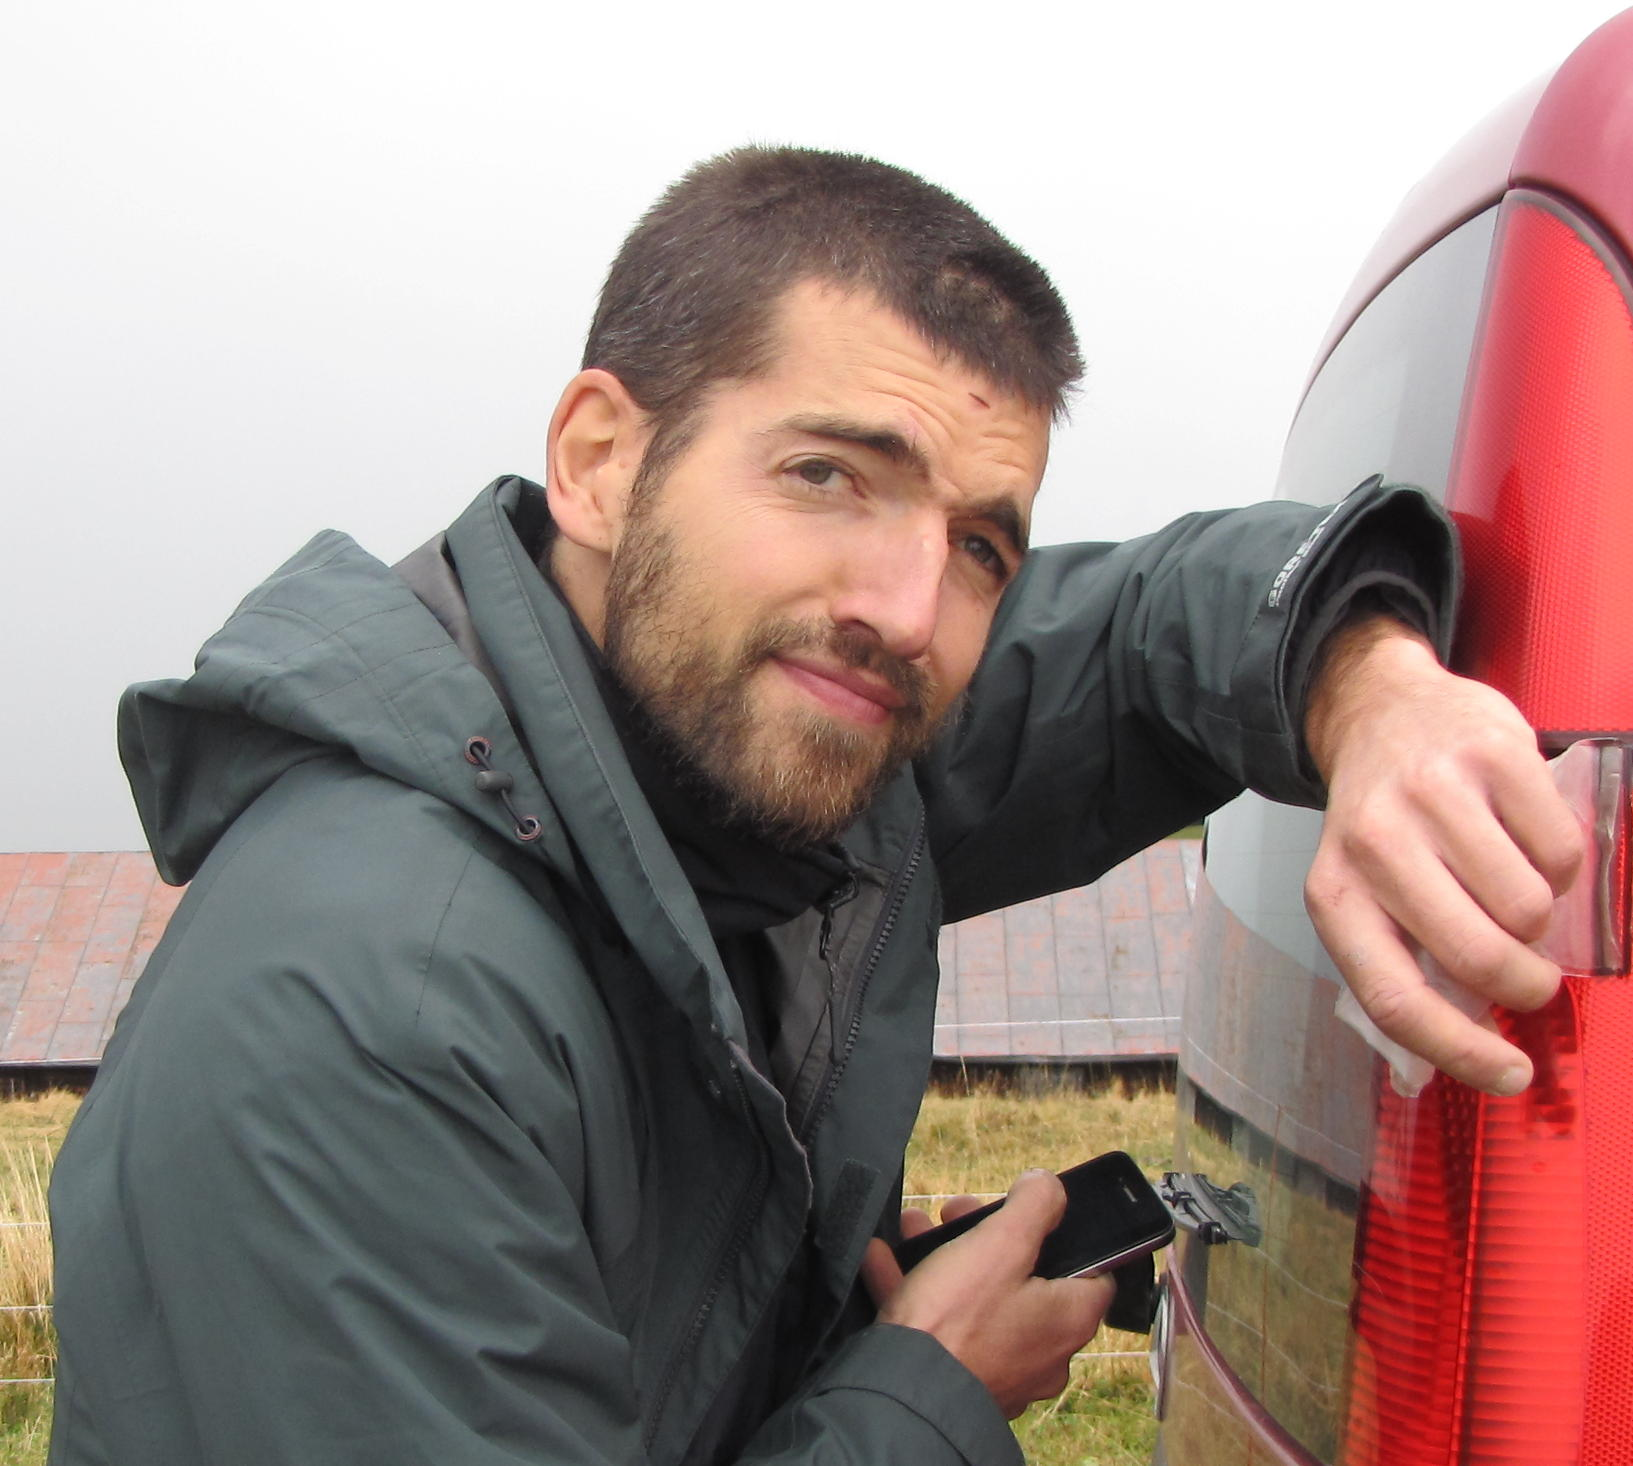
\includegraphics[width = 0.22 \textwidth]{Figures/Glauco}};}
				\uncover<5->{\node (ursina) at ($(glauco)+(1.2,0)$) {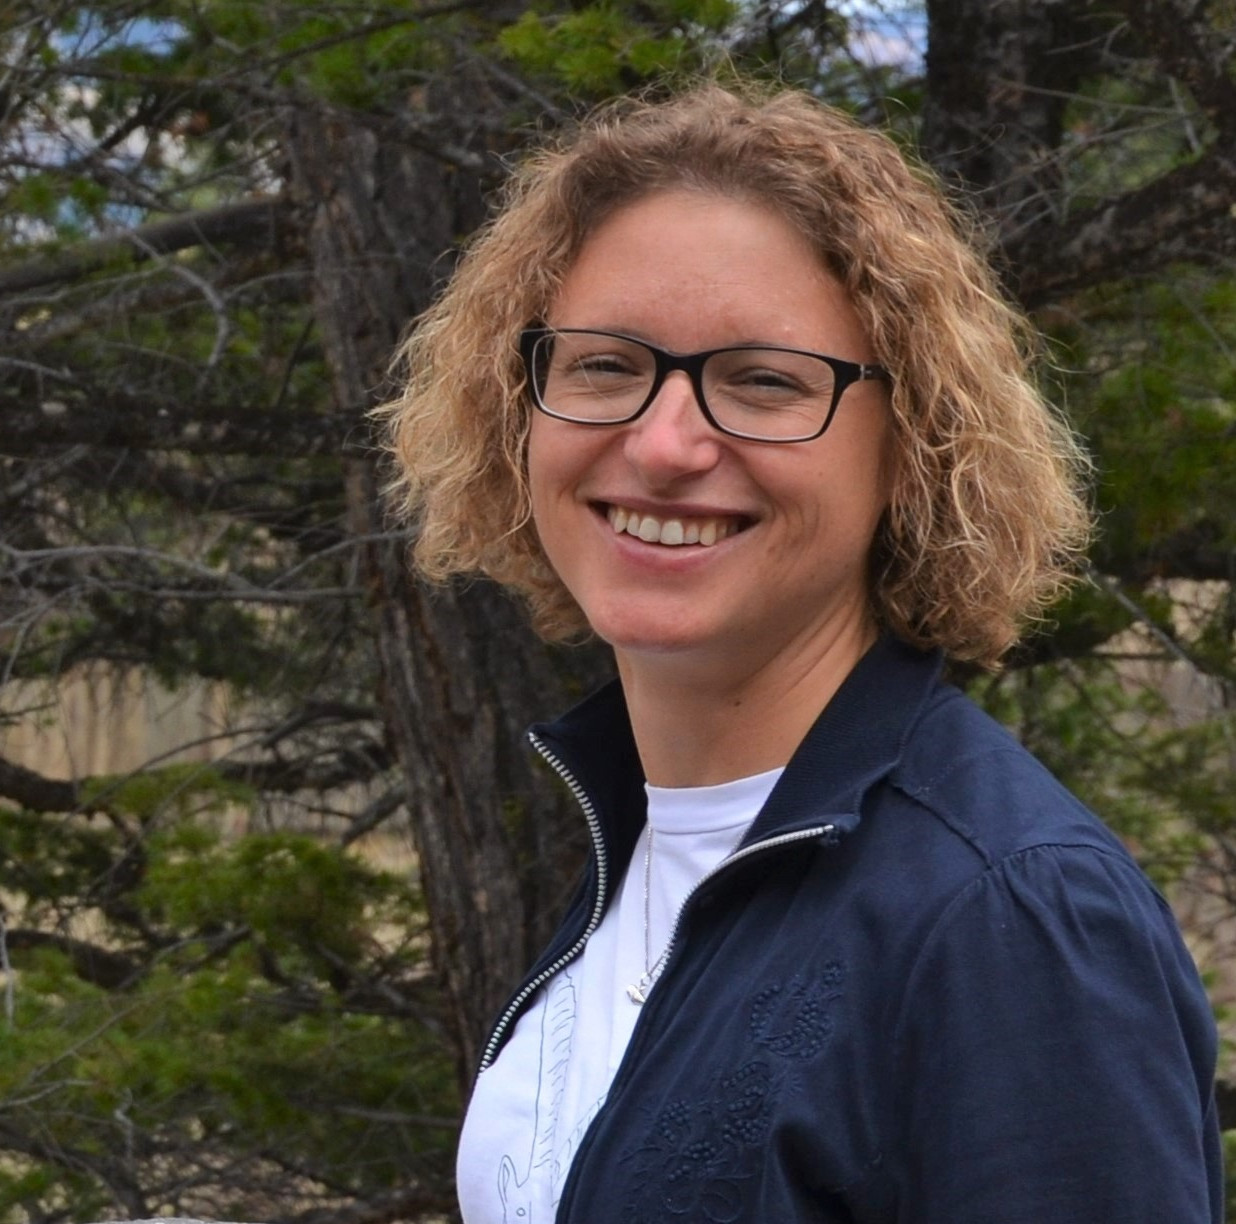
\includegraphics[width = 0.20 \textwidth]{Figures/Ursina}};}
				\uncover<6->{\node (domi) at ($(ursina)+(1.4,0)$) {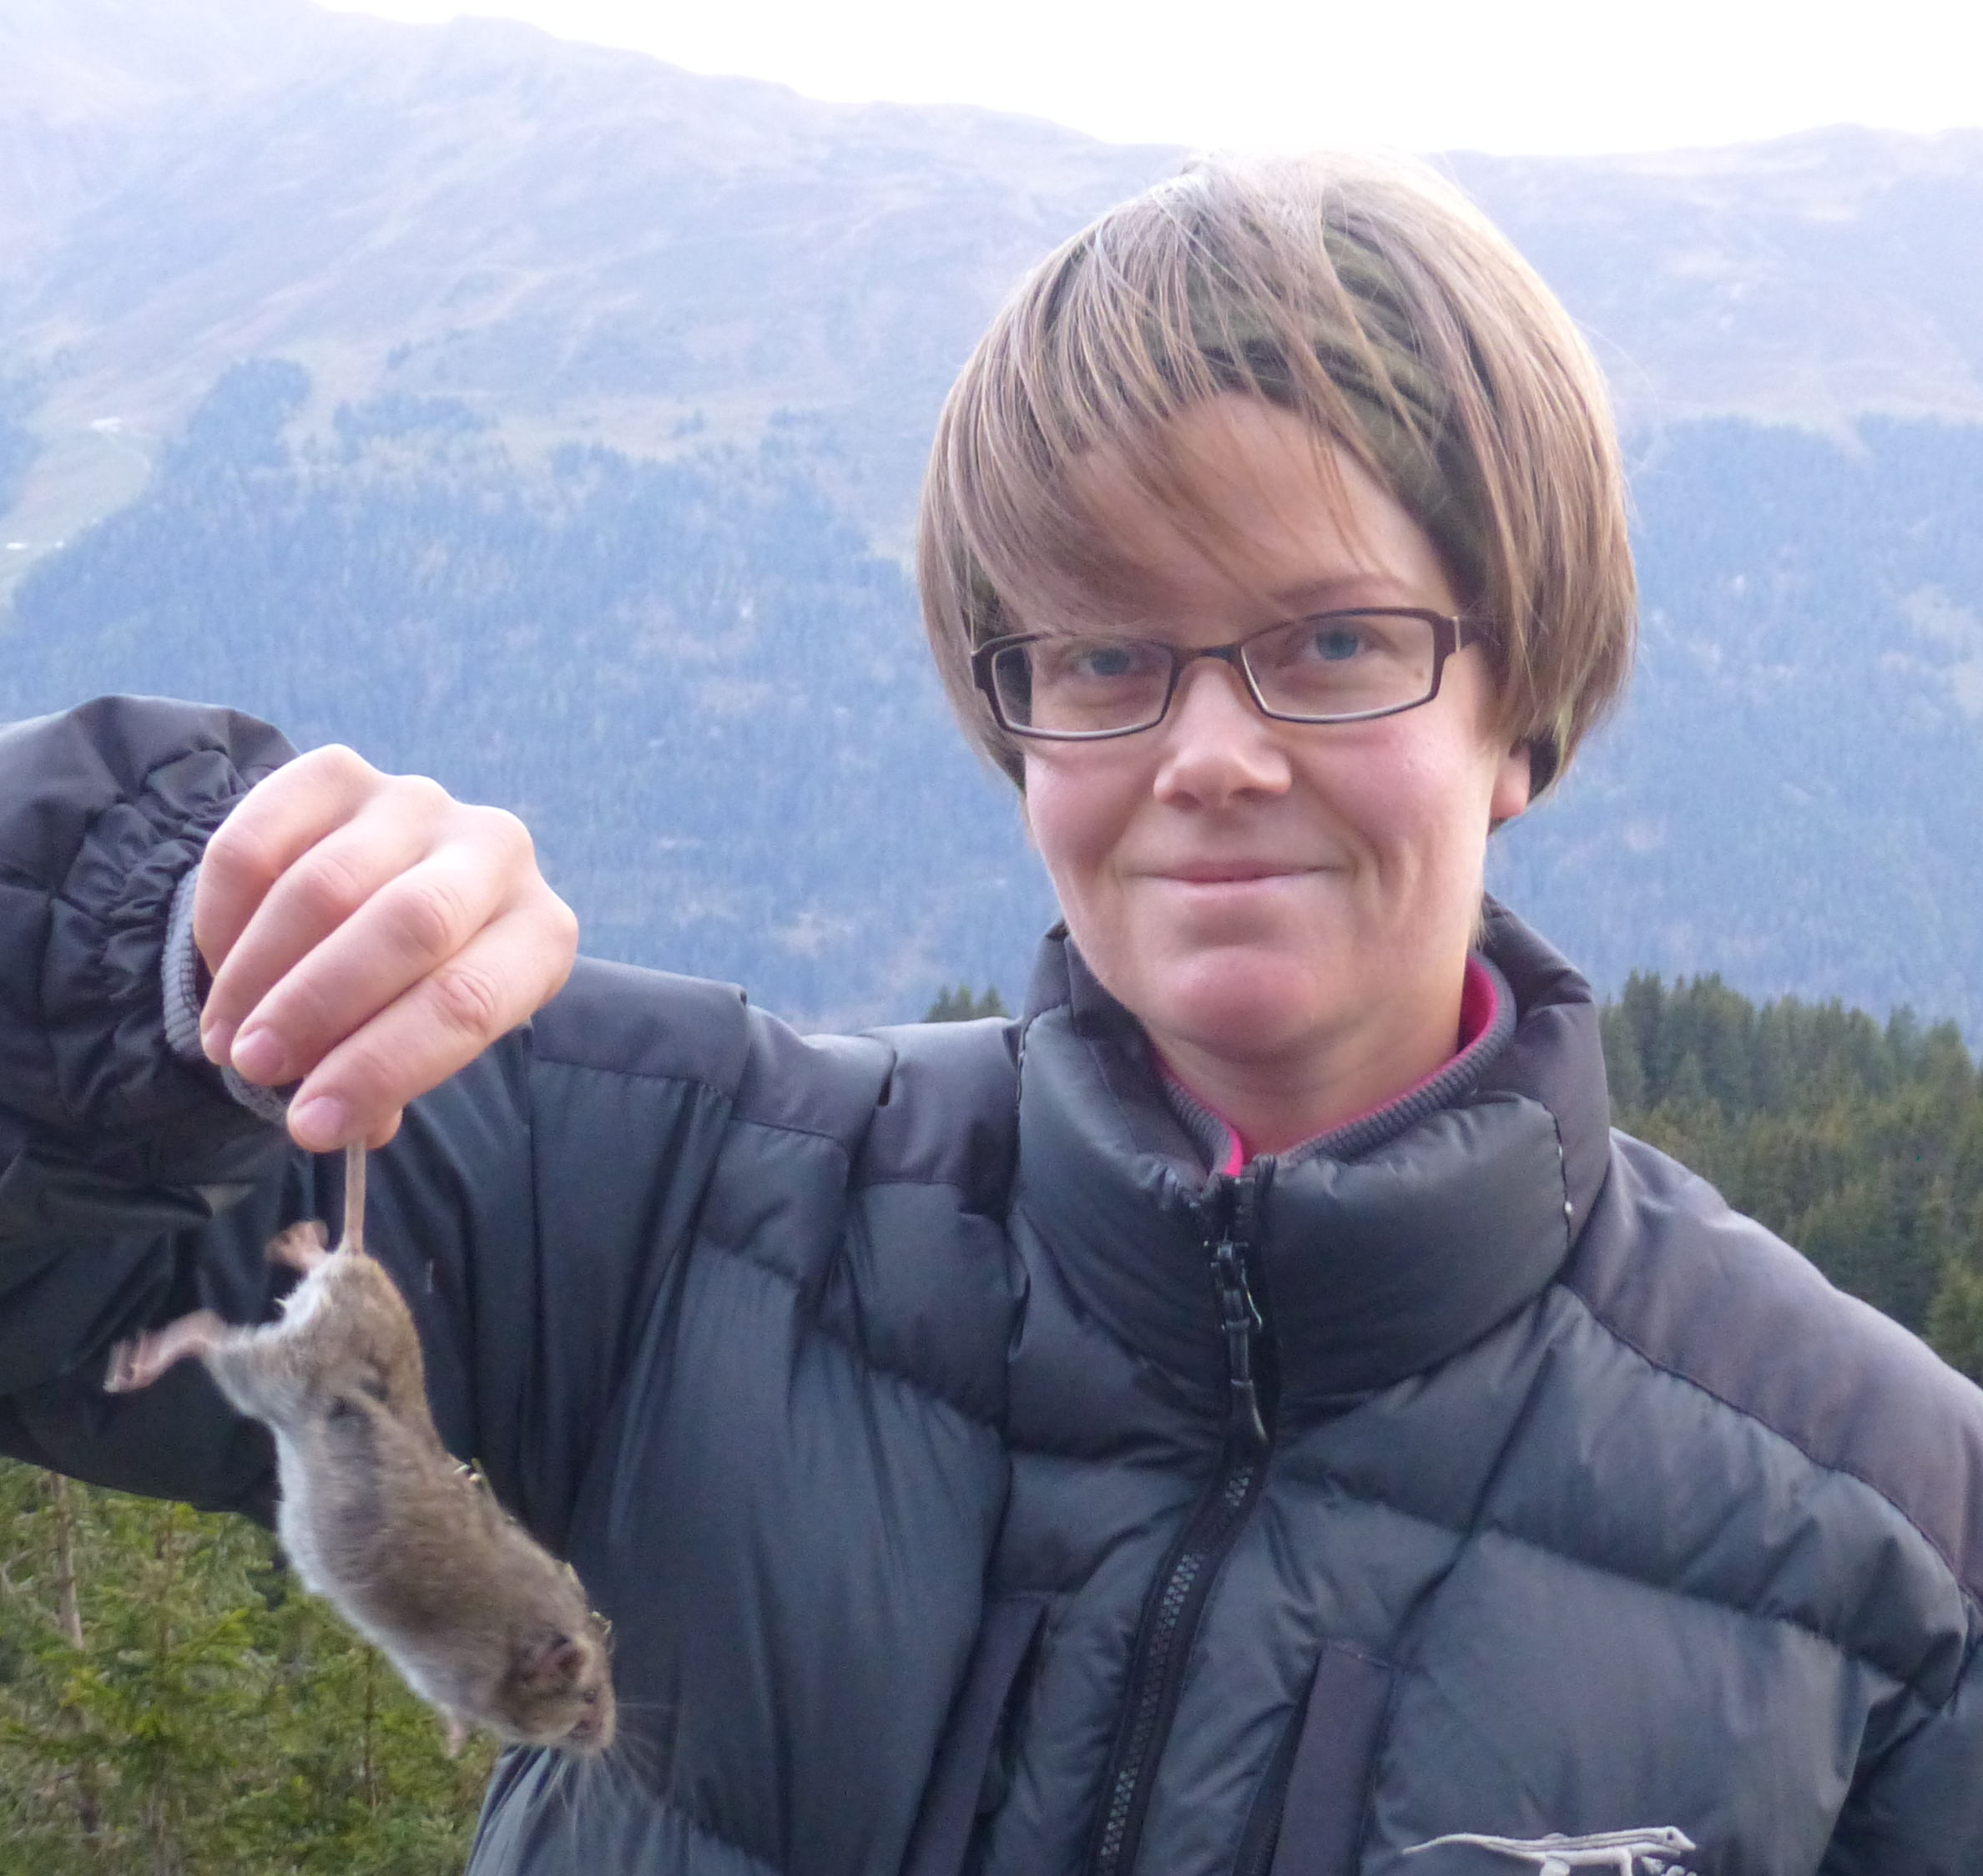
\includegraphics[width = 0.20 \textwidth]{Figures/Domi}};}
				\uncover<6->{\node (martina) at ($(domi)+(1.2,0)$) {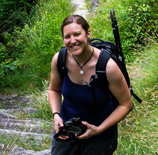
\includegraphics[width = 0.17 \textwidth]{Figures/Martina}};}
				\uncover<6->{\node (vicente) at ($(martina)+(1.2,-0.2)$) {\includegraphics[width = 0.16 \textwidth]{Figures/Vicente}};}
				\uncover<7->{\node (andres) at ($(vicente)+(1.2,-0.1)$) {\includegraphics[width = 0.2 \textwidth]{Figures/Andres}};}
				\uncover<8->{\node (koen) at ($(glauco)+(0,-1.4)$) {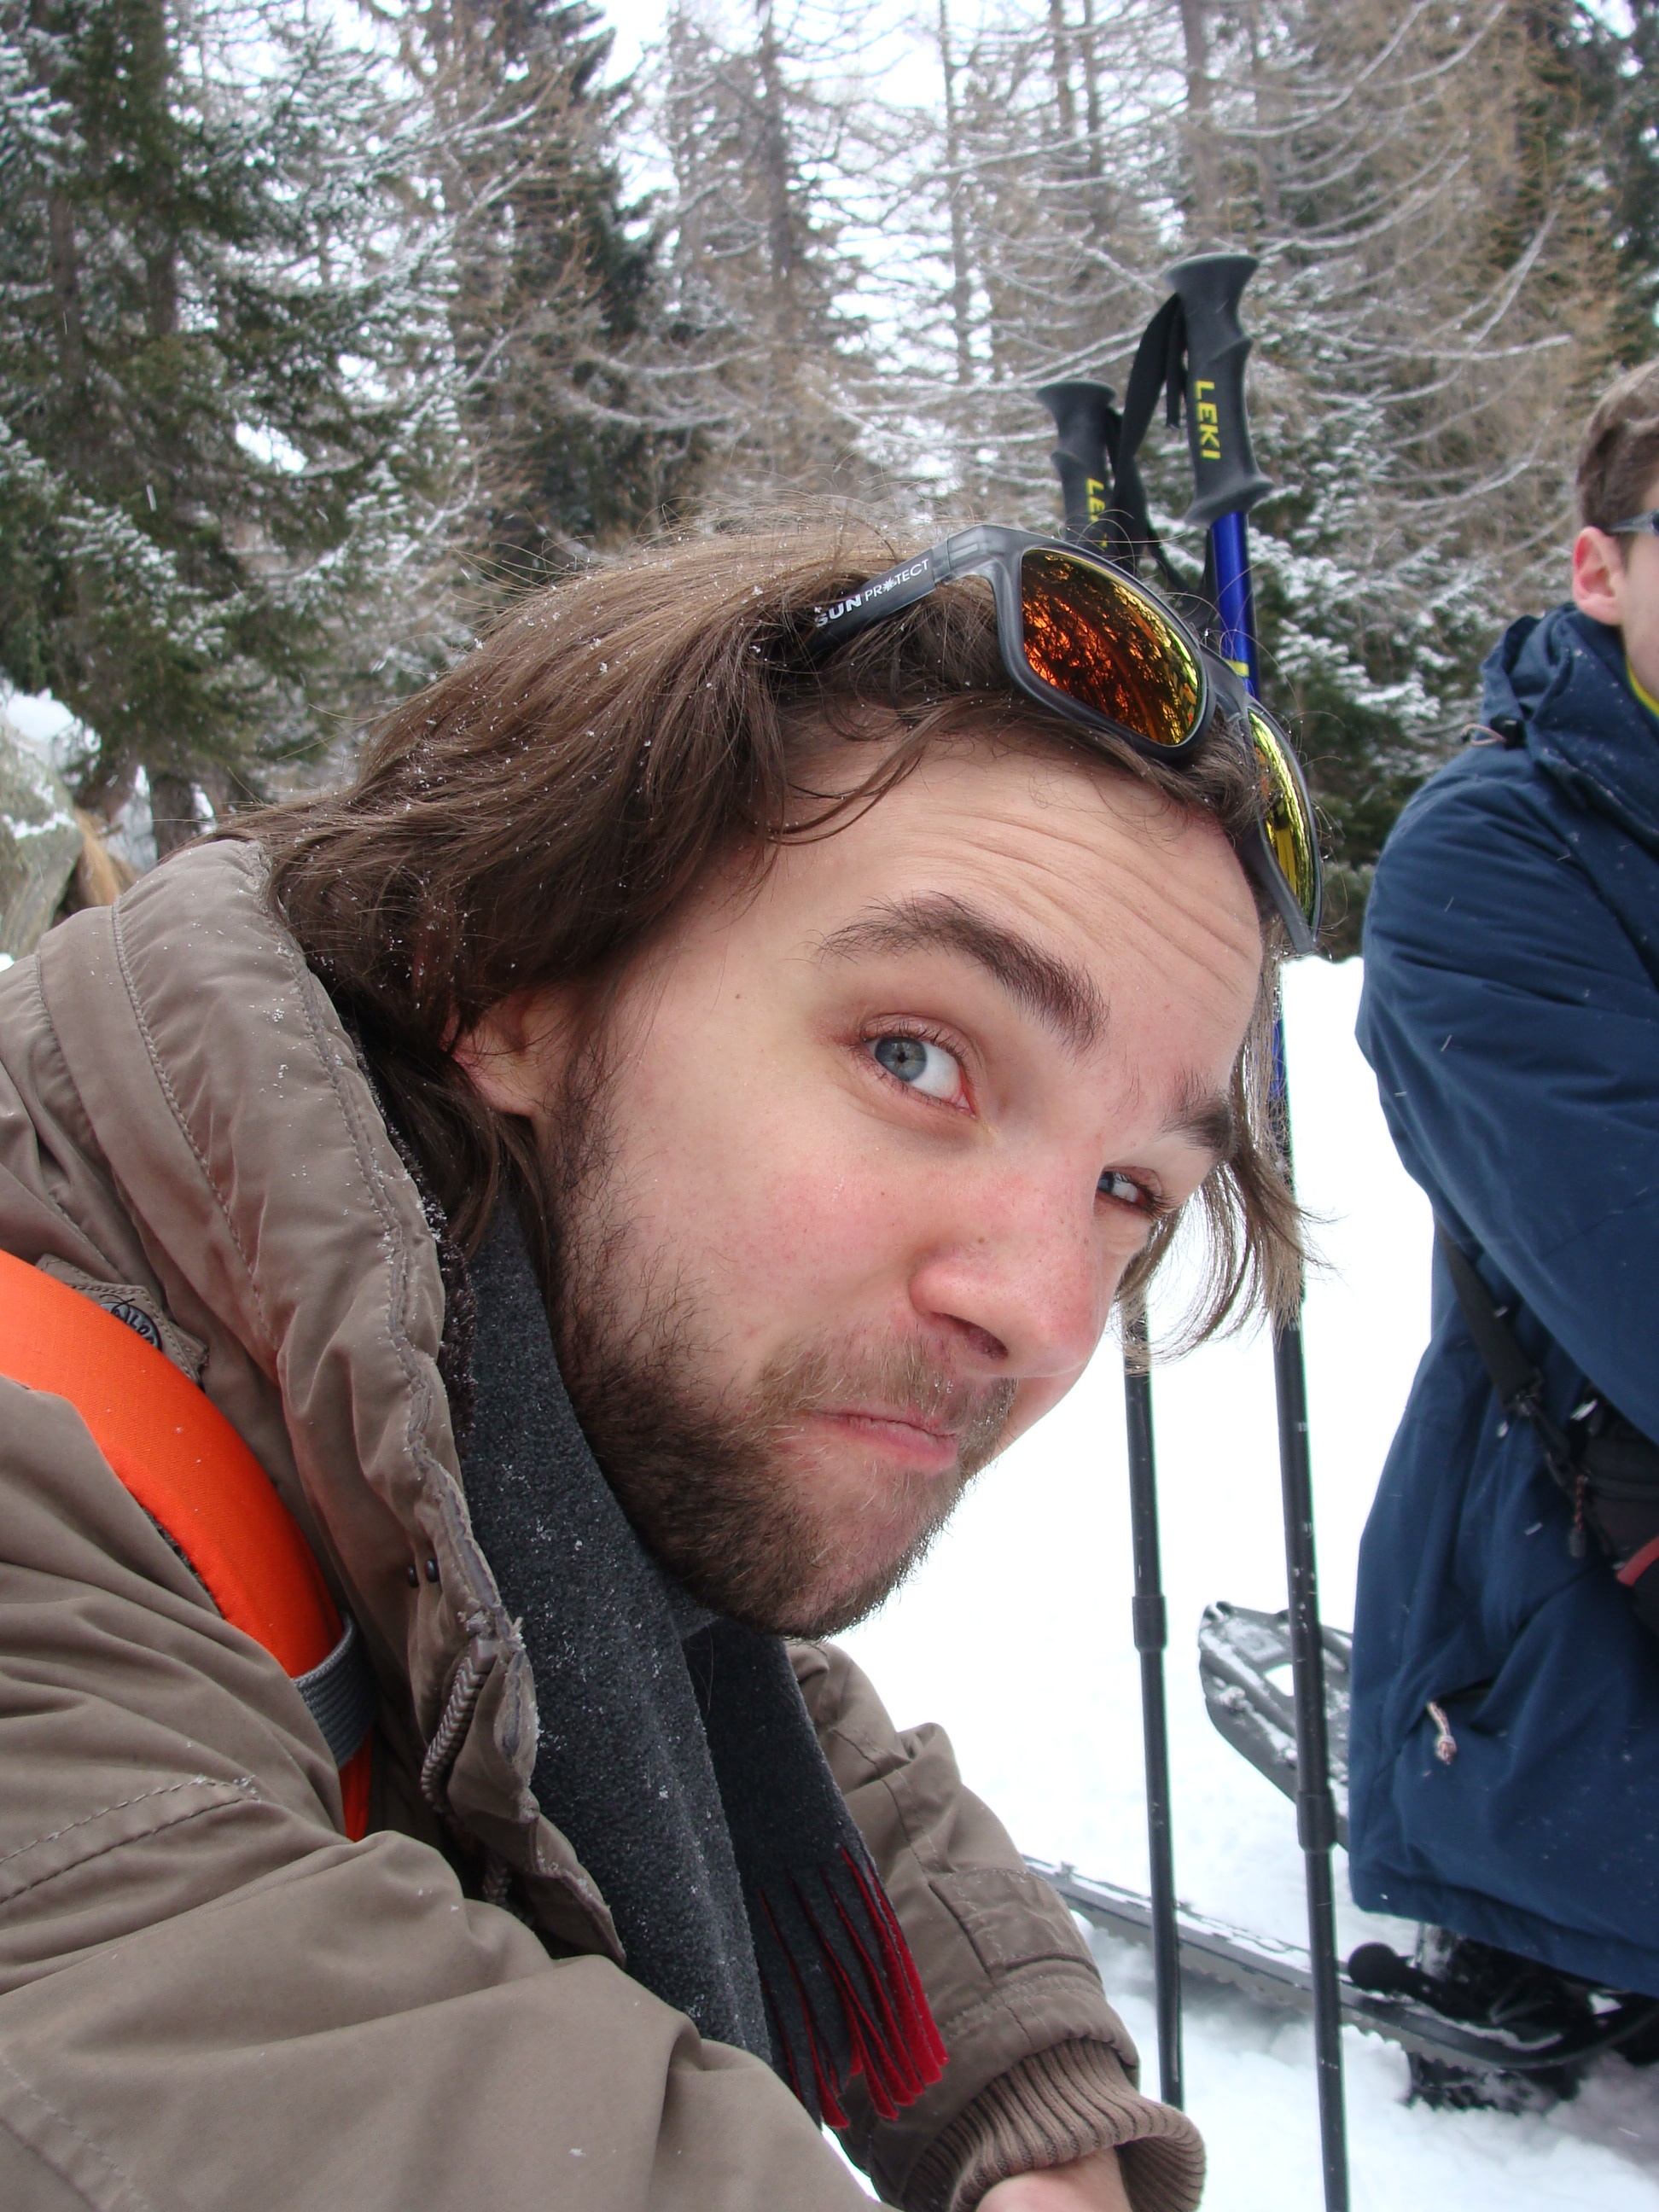
\includegraphics[width = 0.2 \textwidth]{Figures/Koen}};
				\node (marjolein) at ($(koen)+(1.2,0)$) {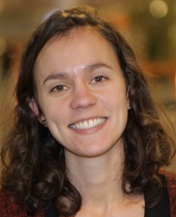
\includegraphics[width = 0.15 \textwidth]{Figures/Marjolein}};
				\node (eelke) at ($(marjolein)+(1.2,0)$) {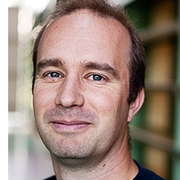
\includegraphics[width = 0.2 \textwidth]{Figures/Eelke}};
				}
				\uncover<9->{
				
				\node (philipp) at ($(eelke)+(1.2,0)$) {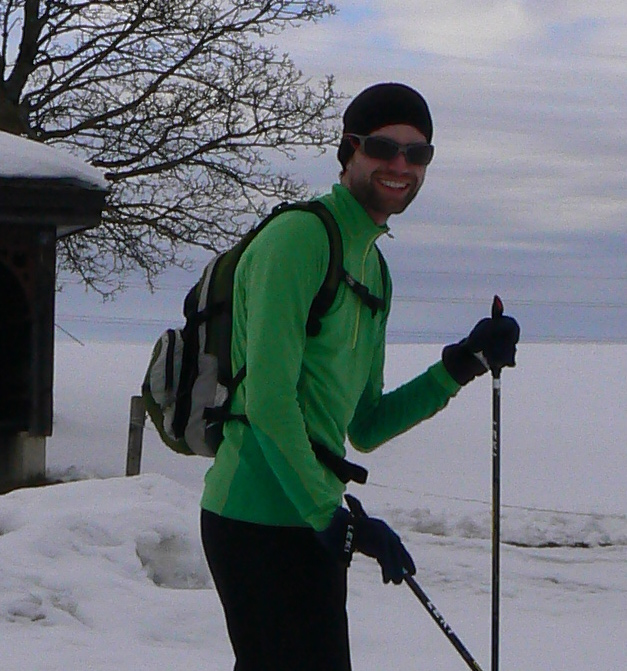
\includegraphics[width = 0.2 \textwidth]{Figures/Philipp}};
				\node (pirmin) at ($(philipp)+(1.2,0)$) {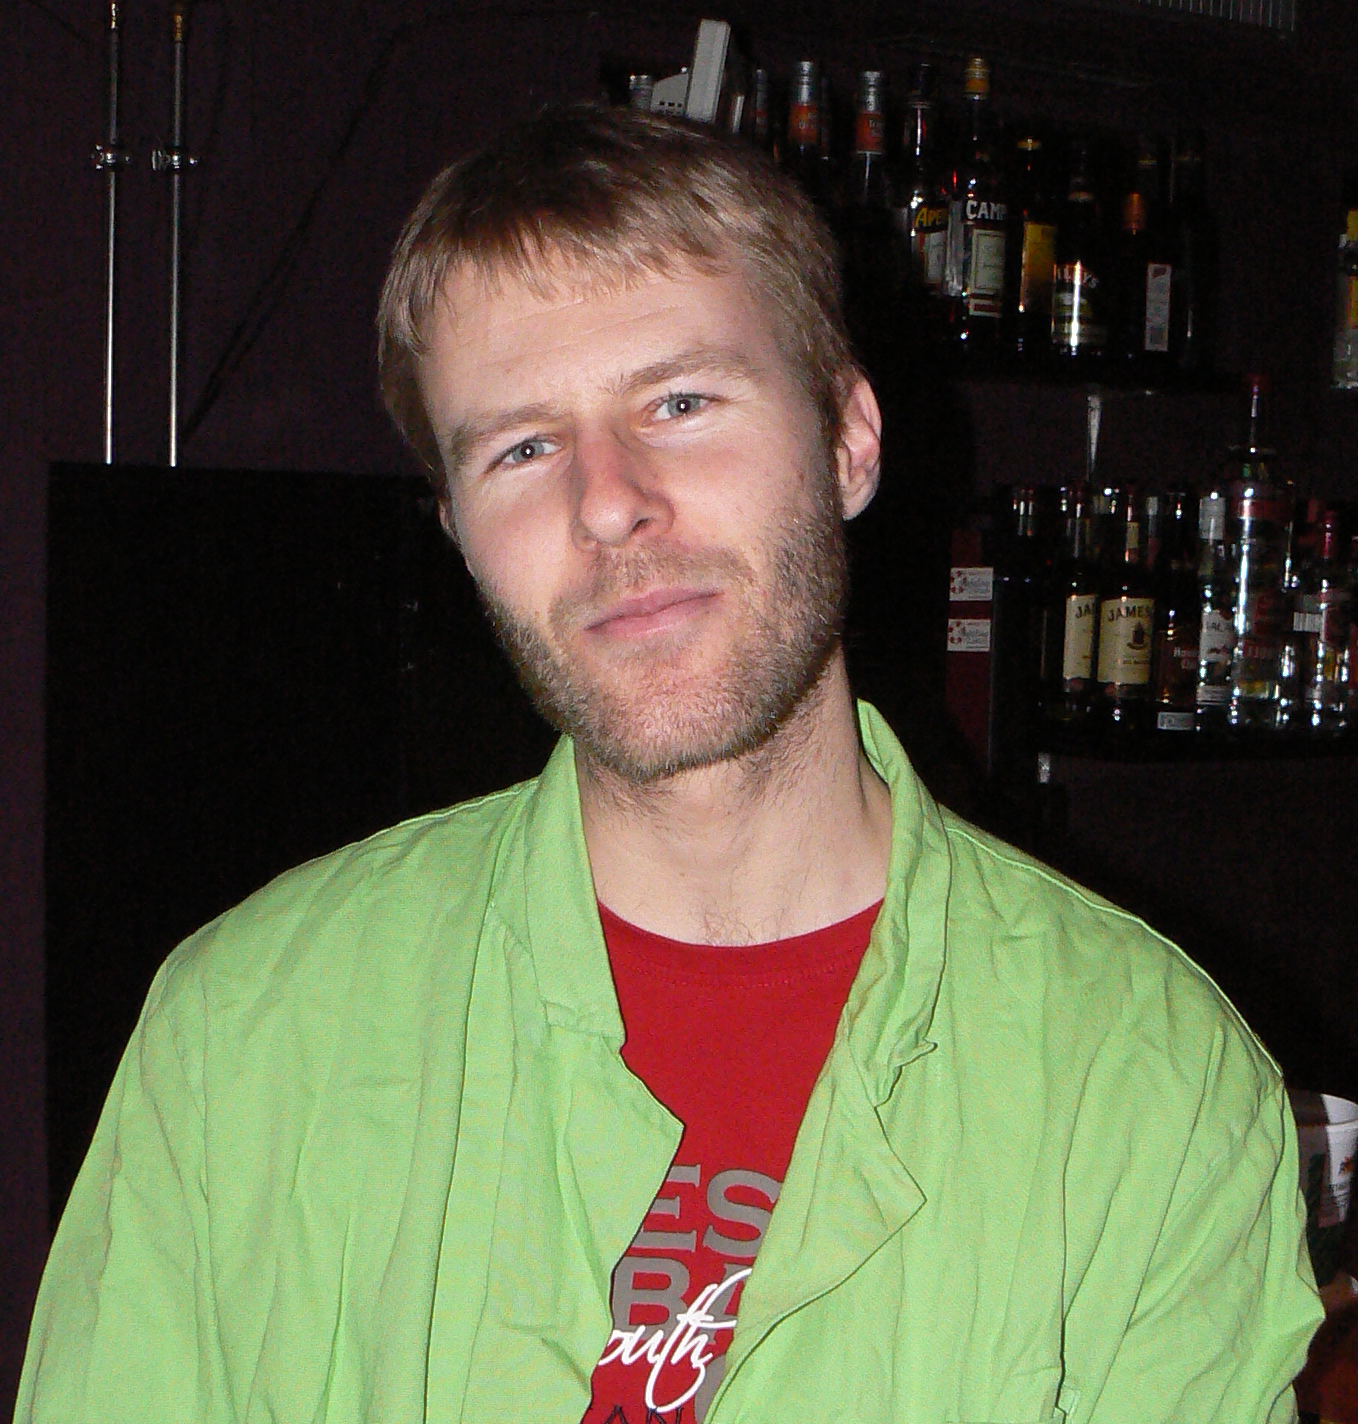
\includegraphics[width = 0.2 \textwidth]{Figures/Pirmin}};
				\node (judith) at ($(pirmin)+(1.2,0)$) {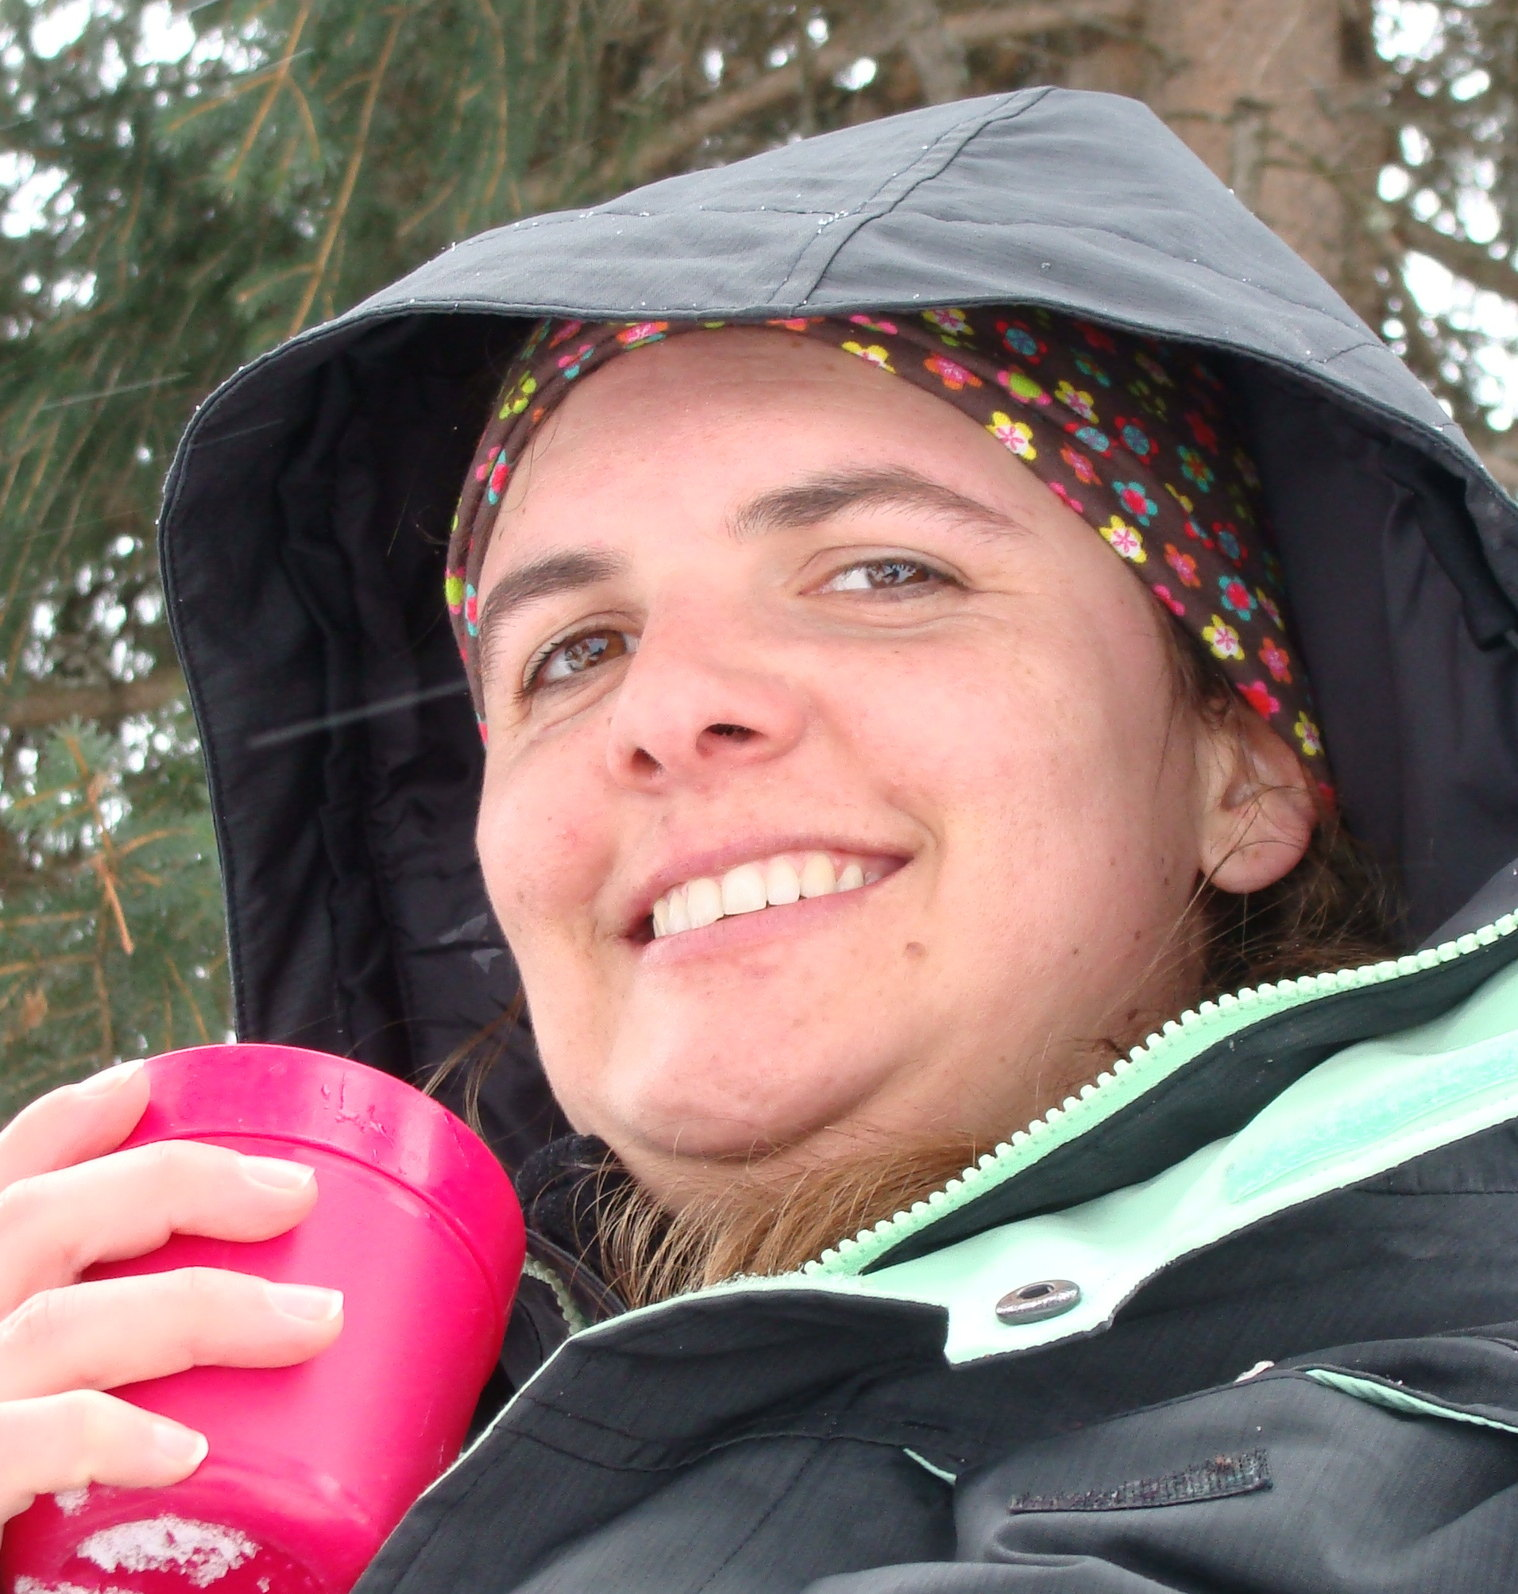
\includegraphics[width = 0.18 \textwidth]{Figures/Judith}};
				}
					\end{tikzpicture}
		\end{figure}
	\end{column}
\end{columns}

\end{frame}
%%%%%%%%%%%

\begin{frame}[plain]
\begin{columns}
\begin{column}[c]{0.7\textwidth}
		\begin{figure}[c]
			\begin{tikzpicture}

							\node (erik) at (0,0) {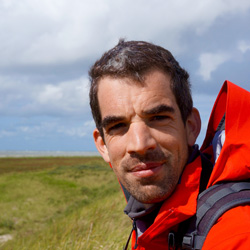
\includegraphics[width = 0.2 \textwidth]{Figures/Erik}};
				\node (lukas) at ($(erik)+(1.2,0)$) {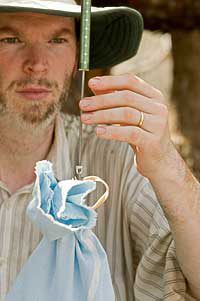
\includegraphics[width = 0.15 \textwidth]{Figures/Lukas}};
				\node (barbara) at ($(lukas)+(1,0)$) {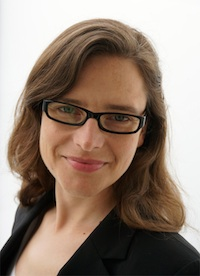
\includegraphics[width = 0.15 \textwidth]{Figures/Barbara}};
				\node (arpat) at ($(barbara)+(1.3,0)$) {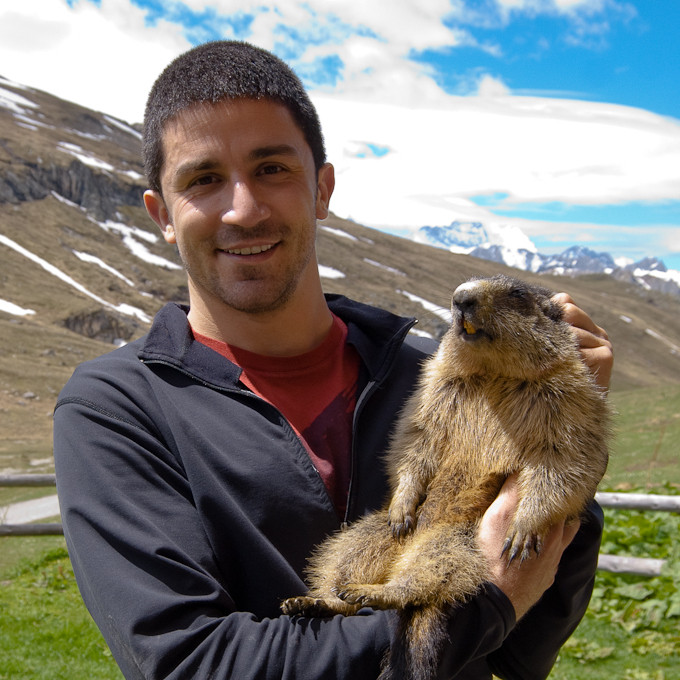
\includegraphics[width = 0.2 \textwidth]{Figures/Arpat}};
				\node (marc) at ($(arpat)+(1.2,0)$) {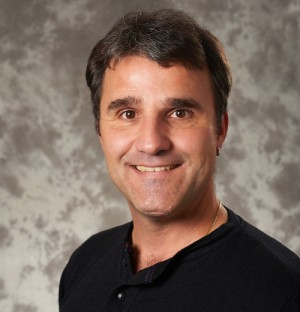
\includegraphics[width = 0.2 \textwidth]{Figures/Marc}};
				\node (jarrod) at ($(marc)+(1.3,0)$) {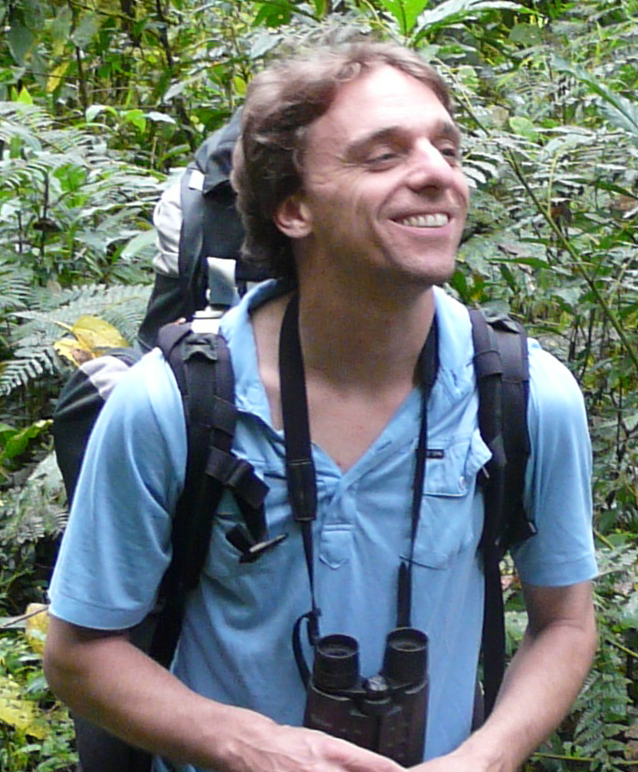
\includegraphics[width = 0.2\textwidth]{Figures/Jarrod}};
				\node (glauco) at ($(erik)+(0,-1.4)$) {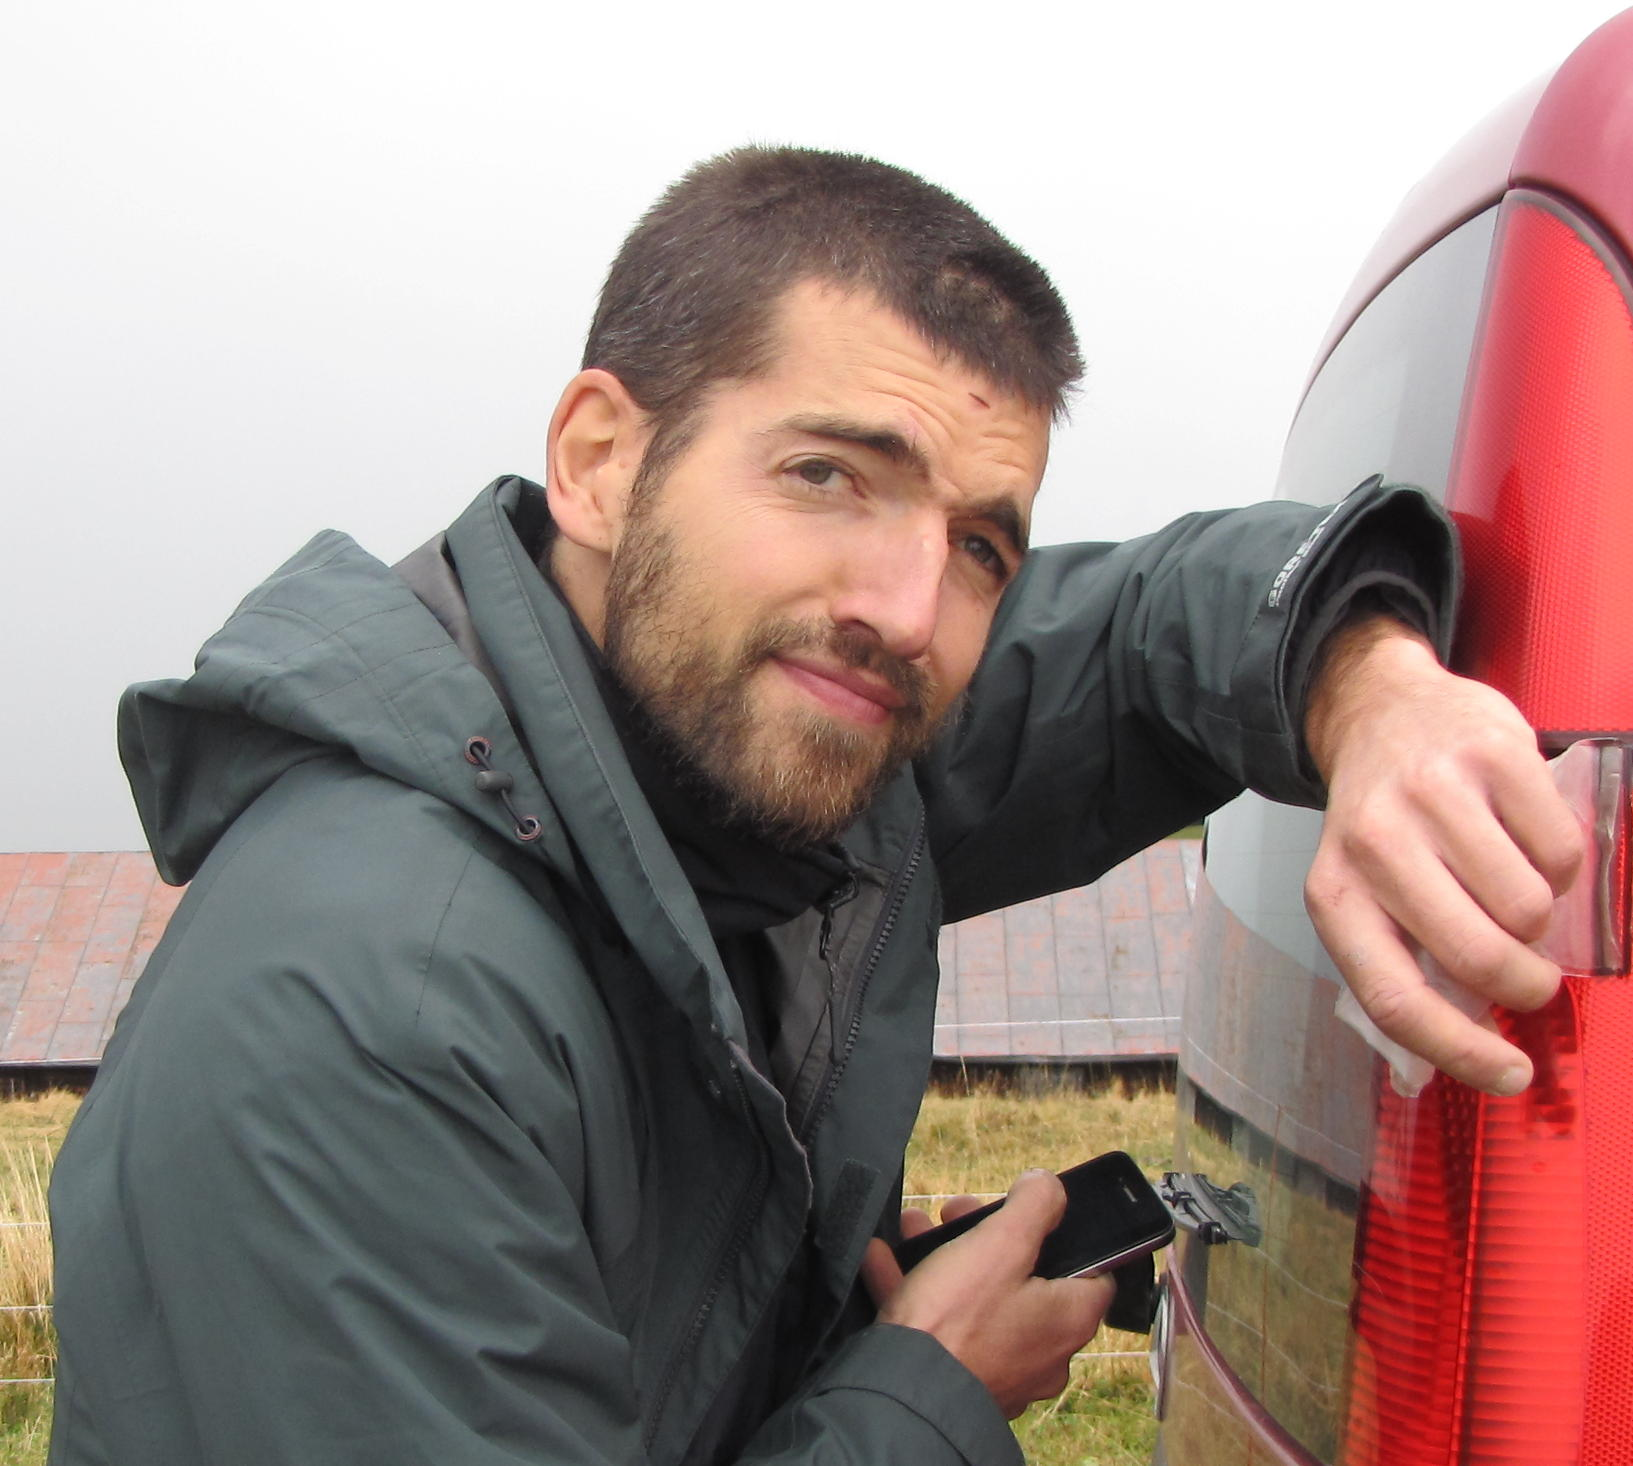
\includegraphics[width = 0.22 \textwidth]{Figures/Glauco}};
			\node (ursina) at ($(glauco)+(1.2,0)$) {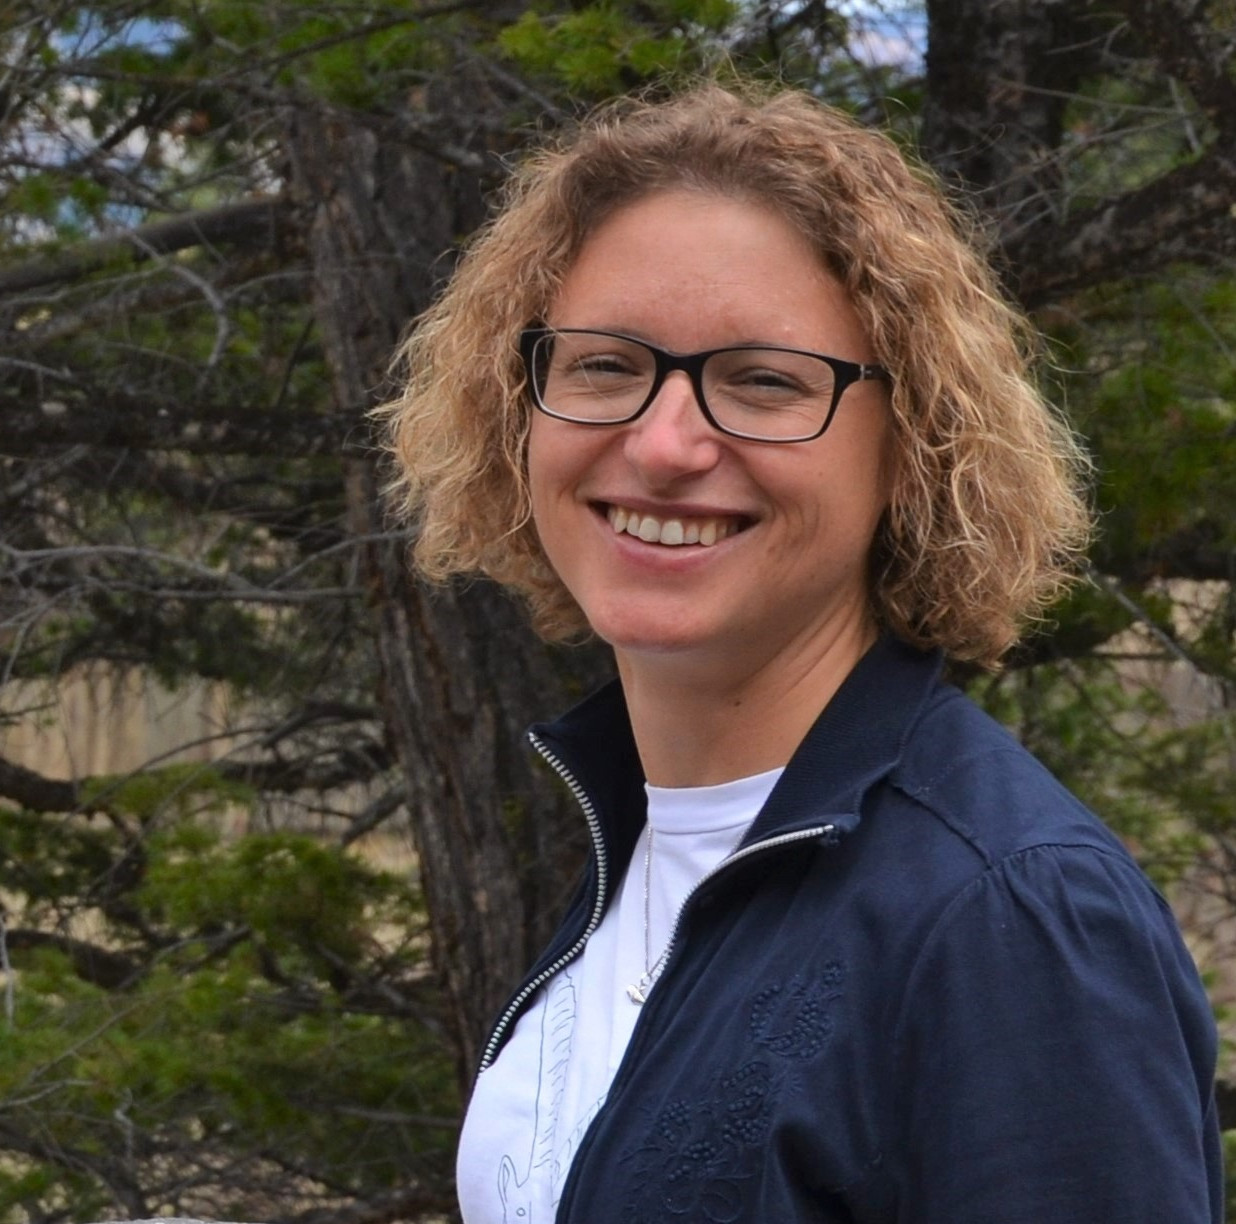
\includegraphics[width = 0.20 \textwidth]{Figures/Ursina}};
				\node (domi) at ($(ursina)+(1.4,0)$) {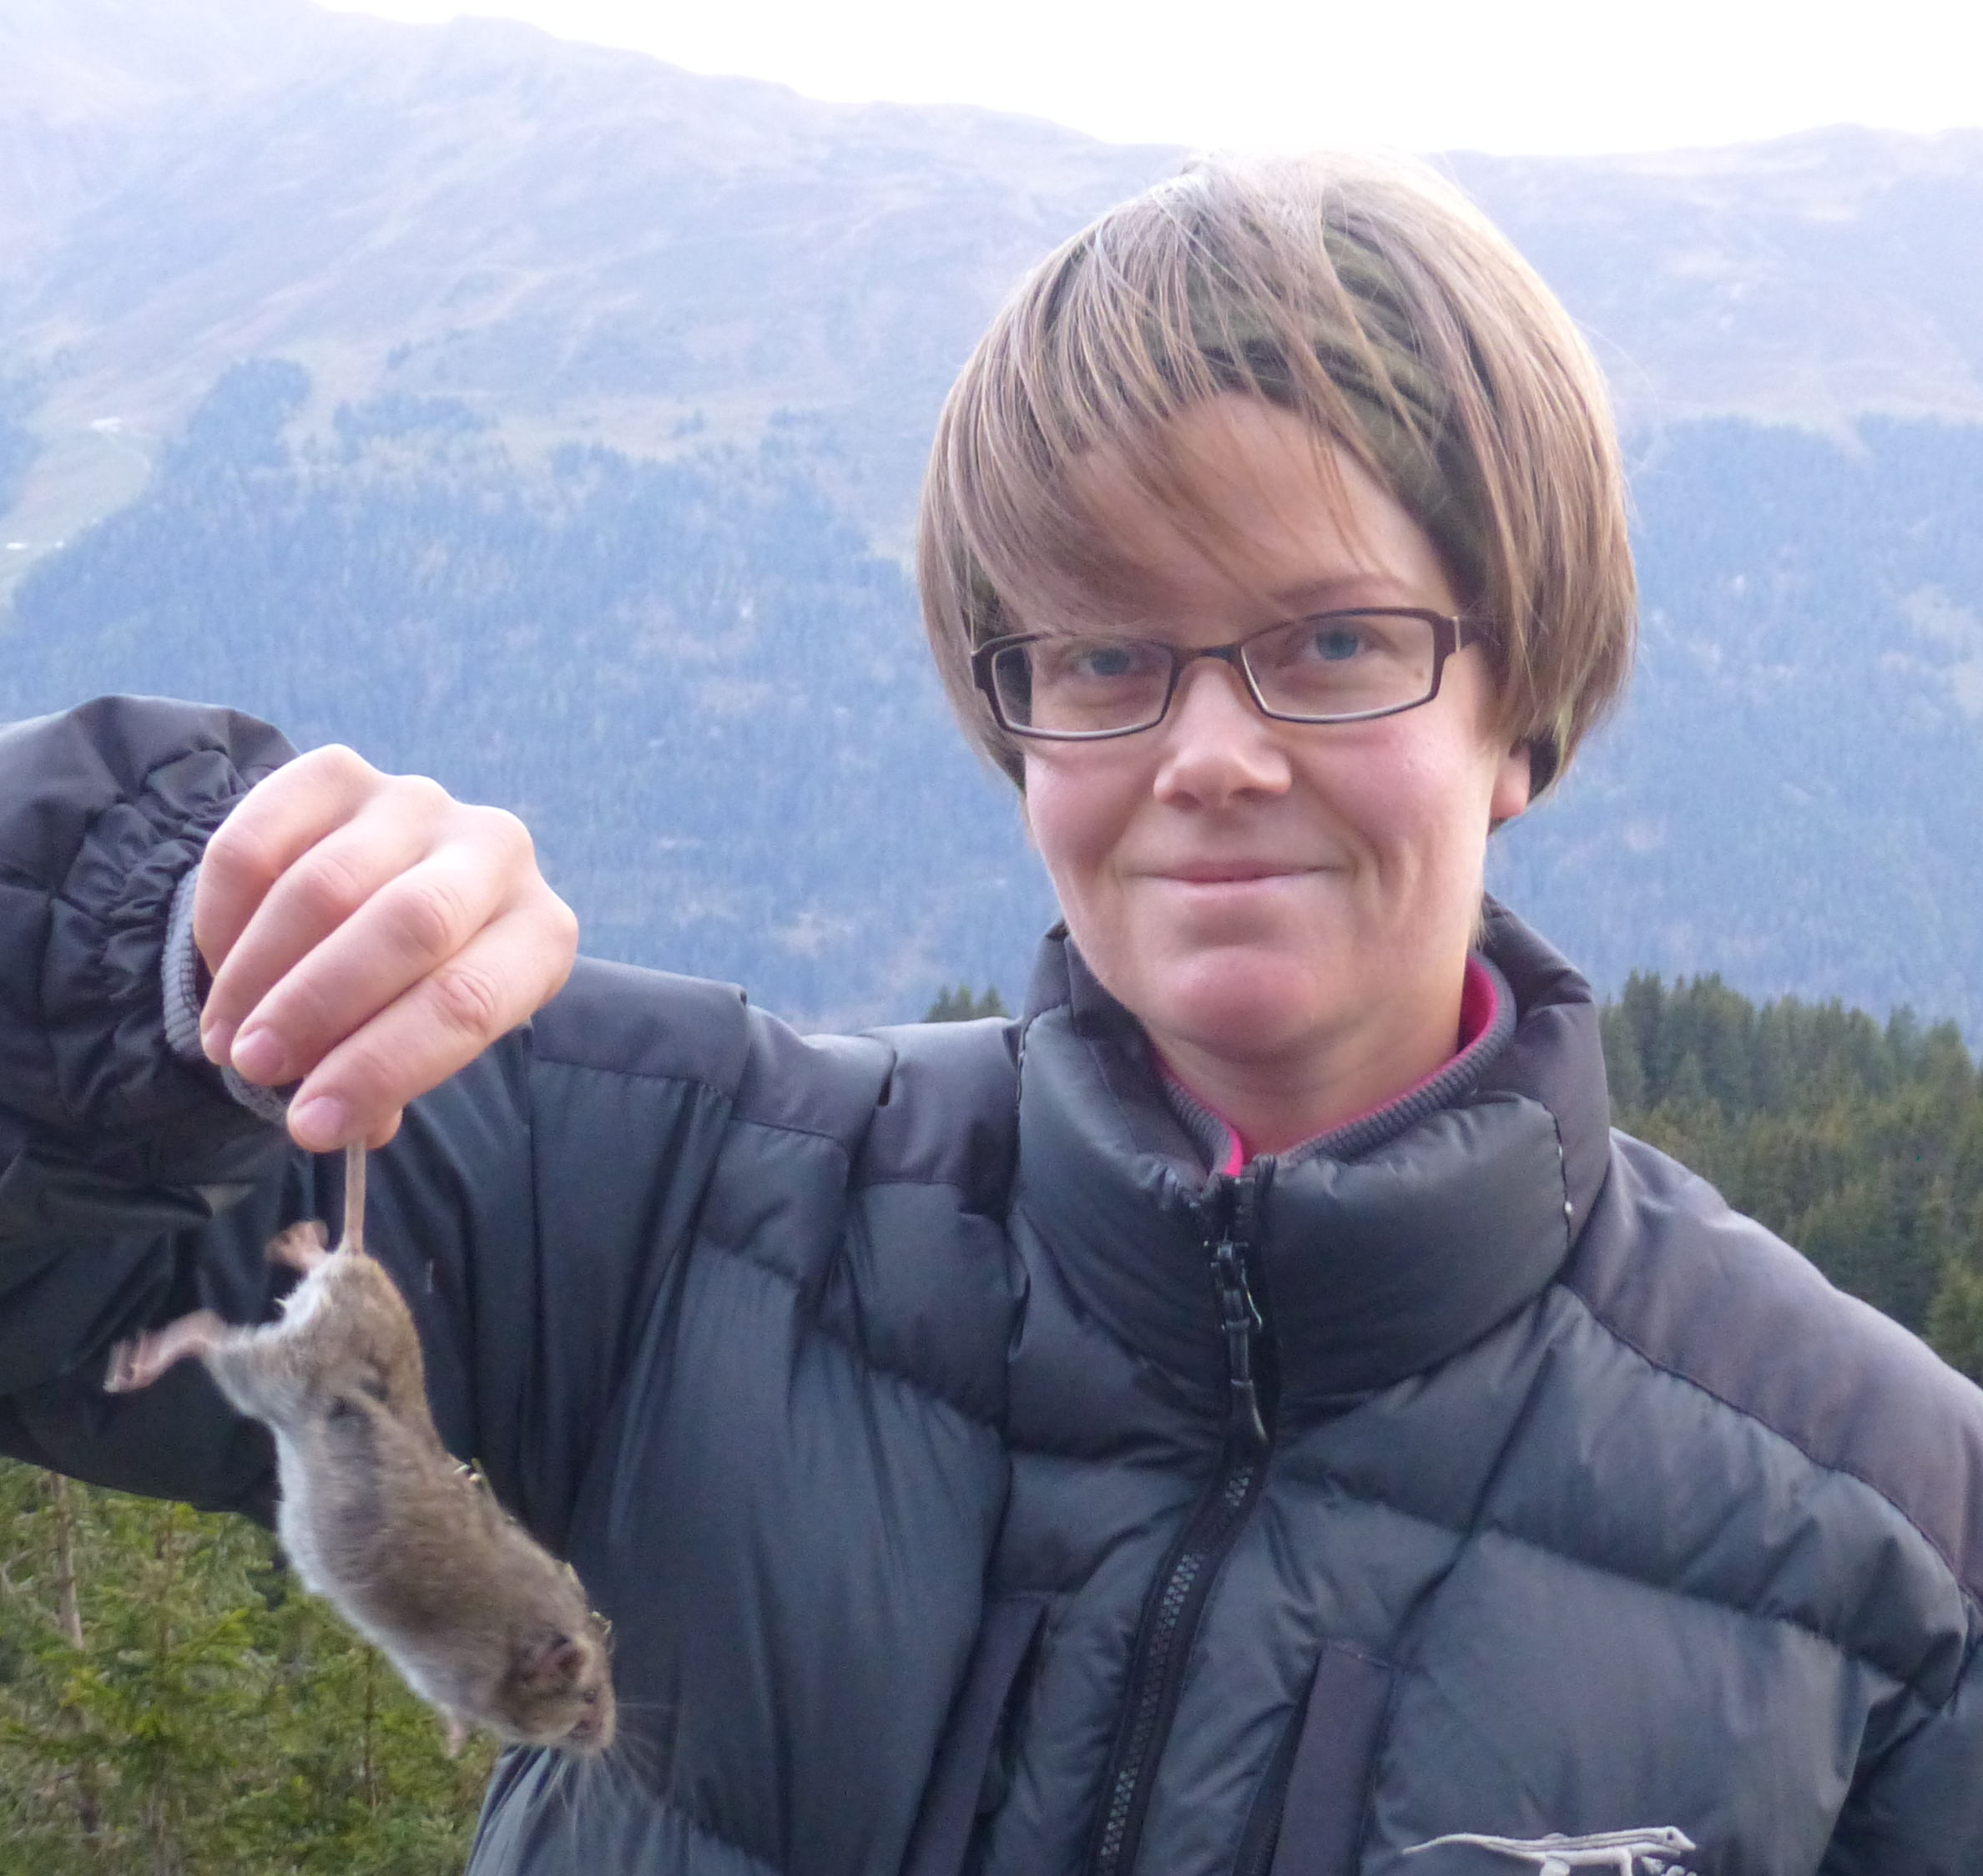
\includegraphics[width = 0.20 \textwidth]{Figures/Domi}};
				\node (martina) at ($(domi)+(1.2,0)$) {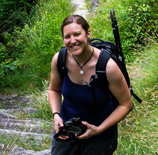
\includegraphics[width = 0.17 \textwidth]{Figures/Martina}};
\node (vicente) at ($(martina)+(1.2,-0.2)$) {\includegraphics[width = 0.16 \textwidth]{Figures/Vicente}};
	\node (andres) at ($(vicente)+(1.2,-0.1)$) {\includegraphics[width = 0.2 \textwidth]{Figures/Andres}};
\node (koen) at ($(glauco)+(0,-1.4)$) {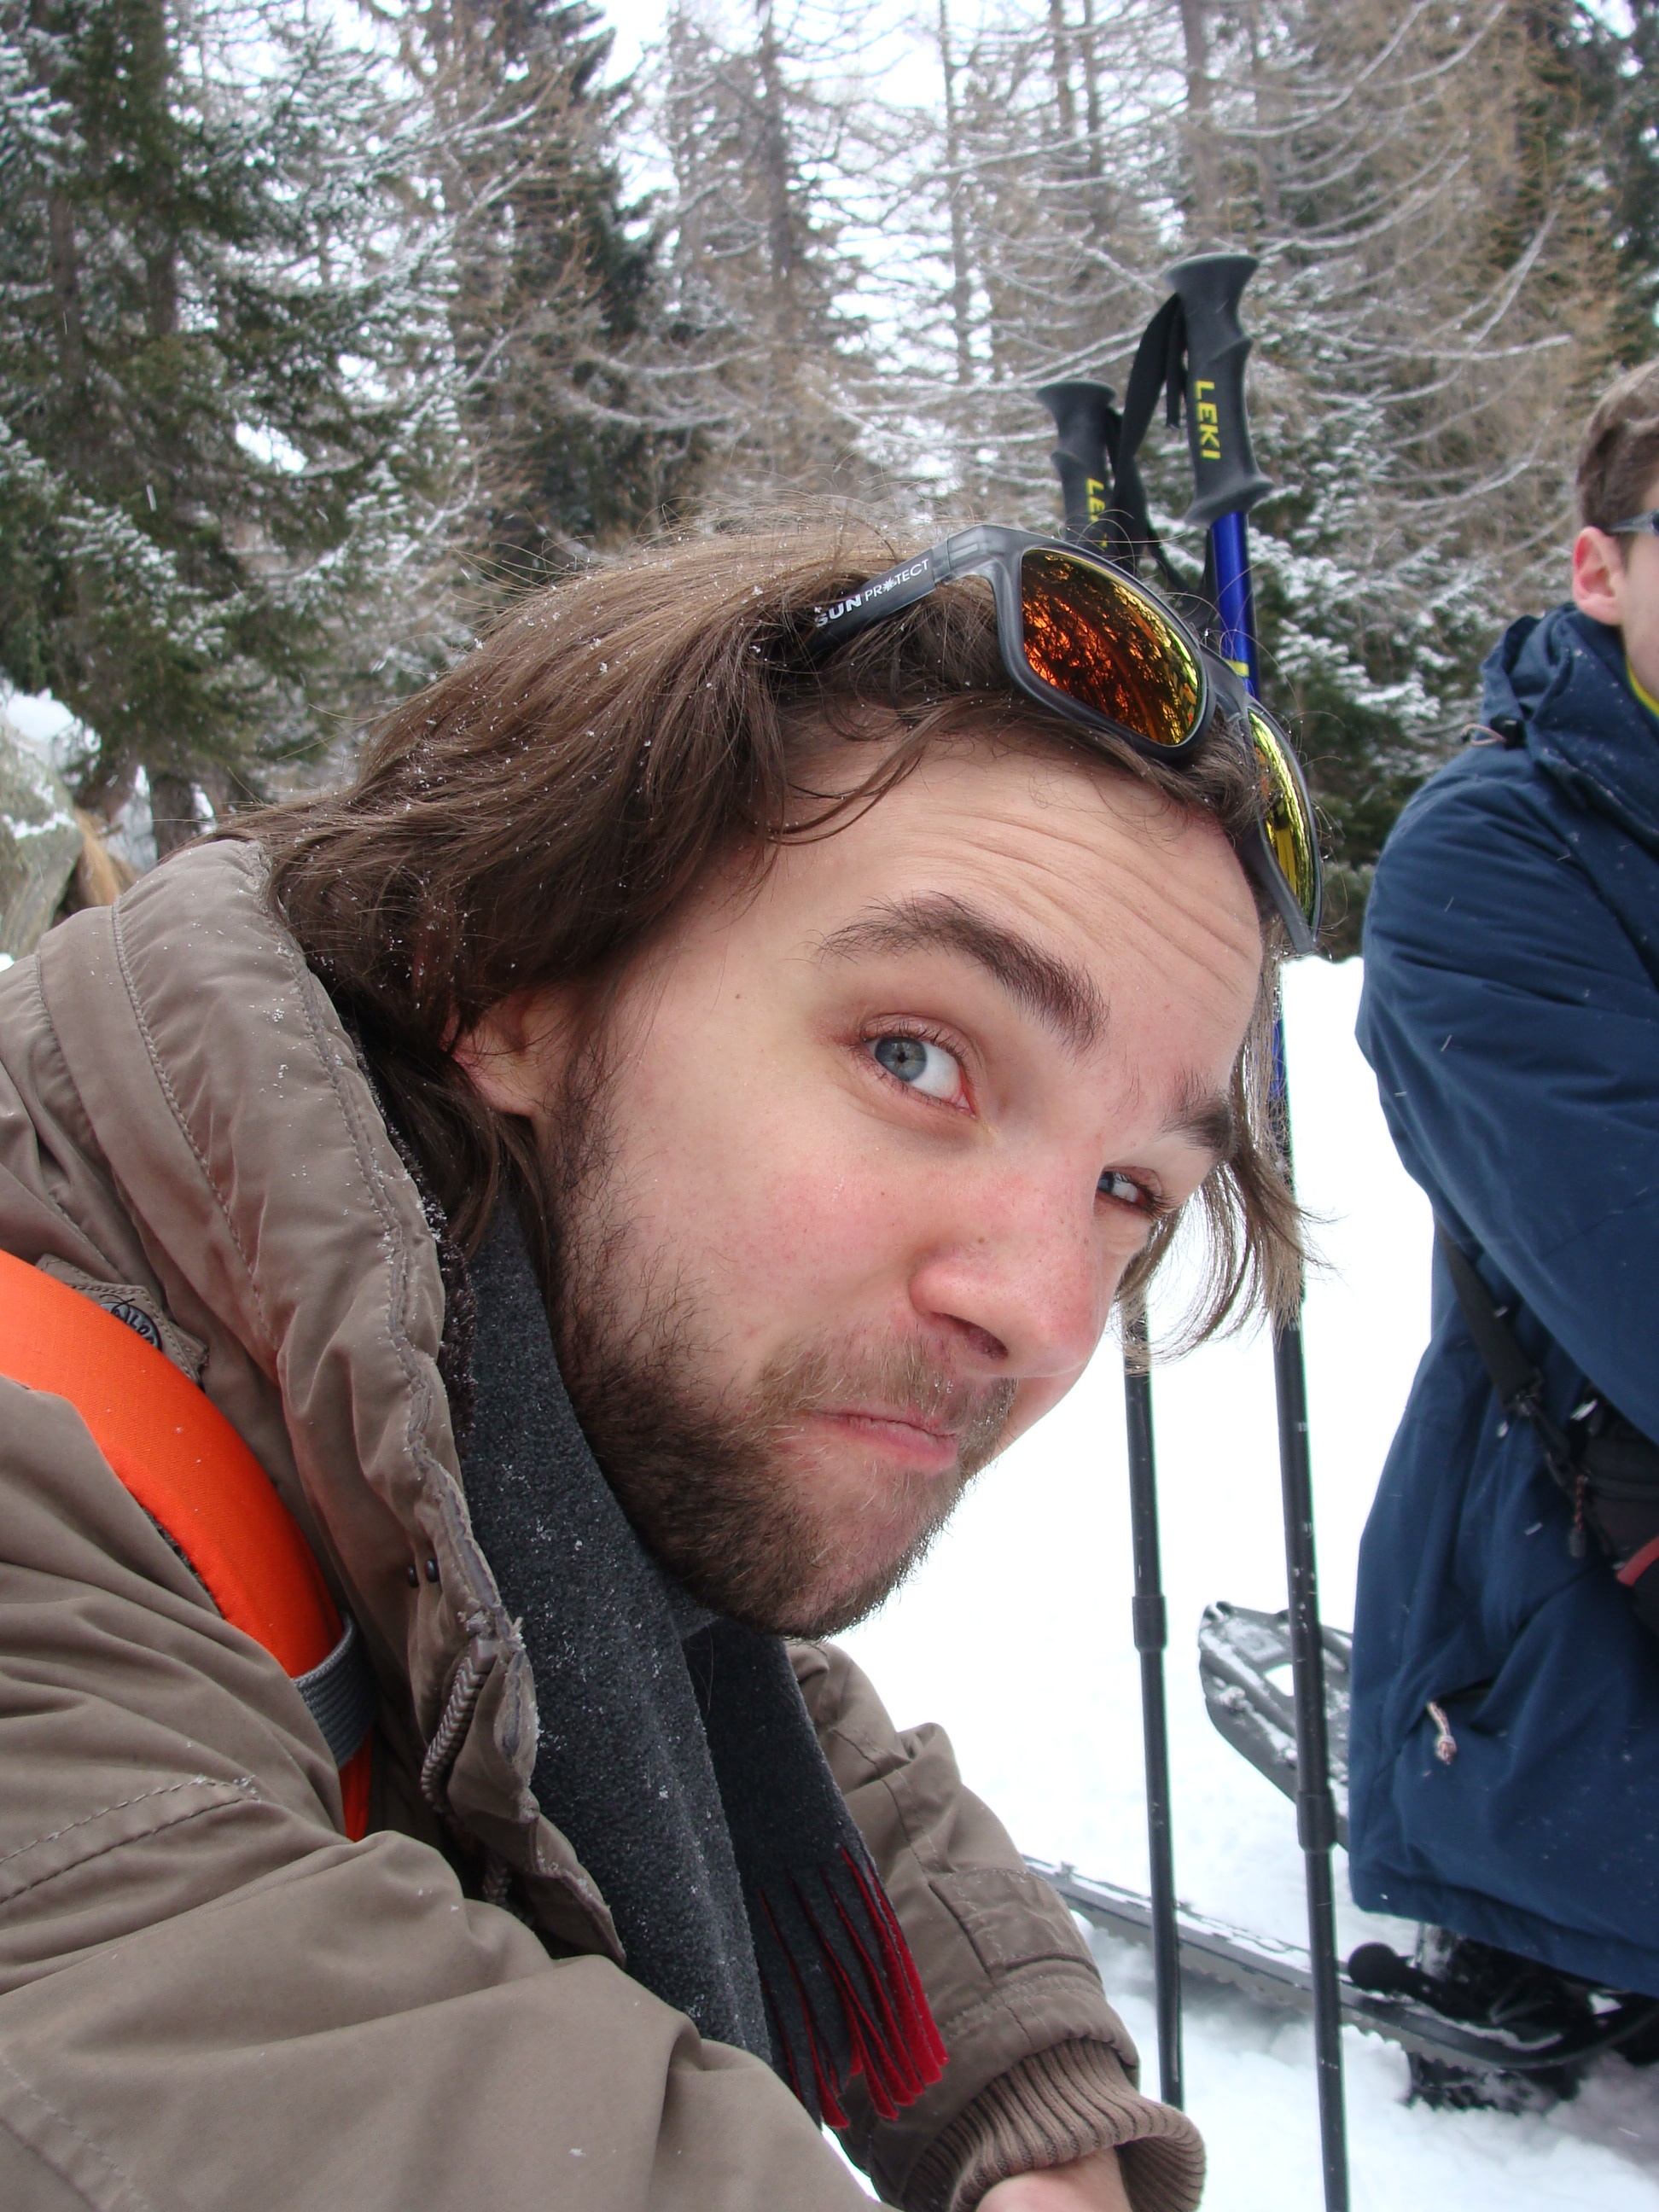
\includegraphics[width = 0.2 \textwidth]{Figures/Koen}};
				\node (marjolein) at ($(koen)+(1.2,0)$) {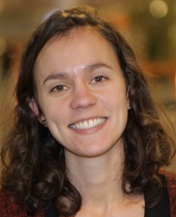
\includegraphics[width = 0.15 \textwidth]{Figures/Marjolein}};
				\node (eelke) at ($(marjolein)+(1.2,0)$) {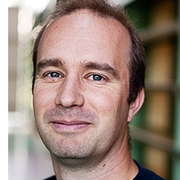
\includegraphics[width = 0.2 \textwidth]{Figures/Eelke}};
				
				
				\node (philipp) at ($(eelke)+(1.2,0)$) {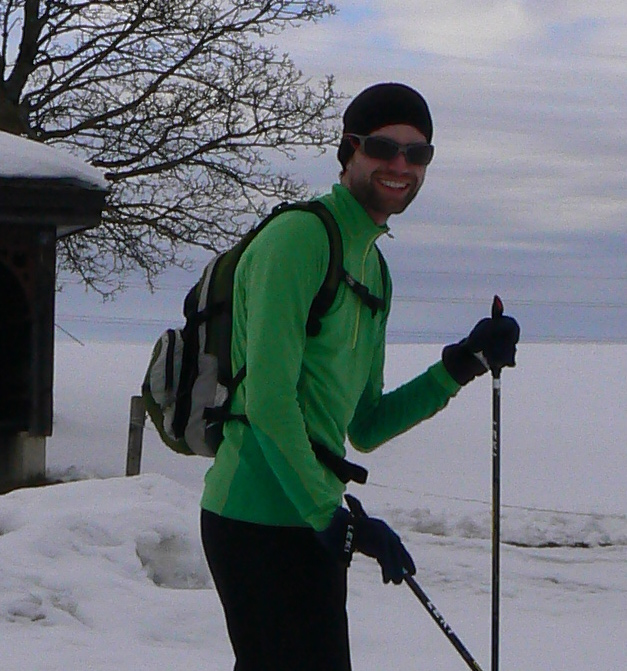
\includegraphics[width = 0.2 \textwidth]{Figures/Philipp}};
				\node (pirmin) at ($(philipp)+(1.2,0)$) {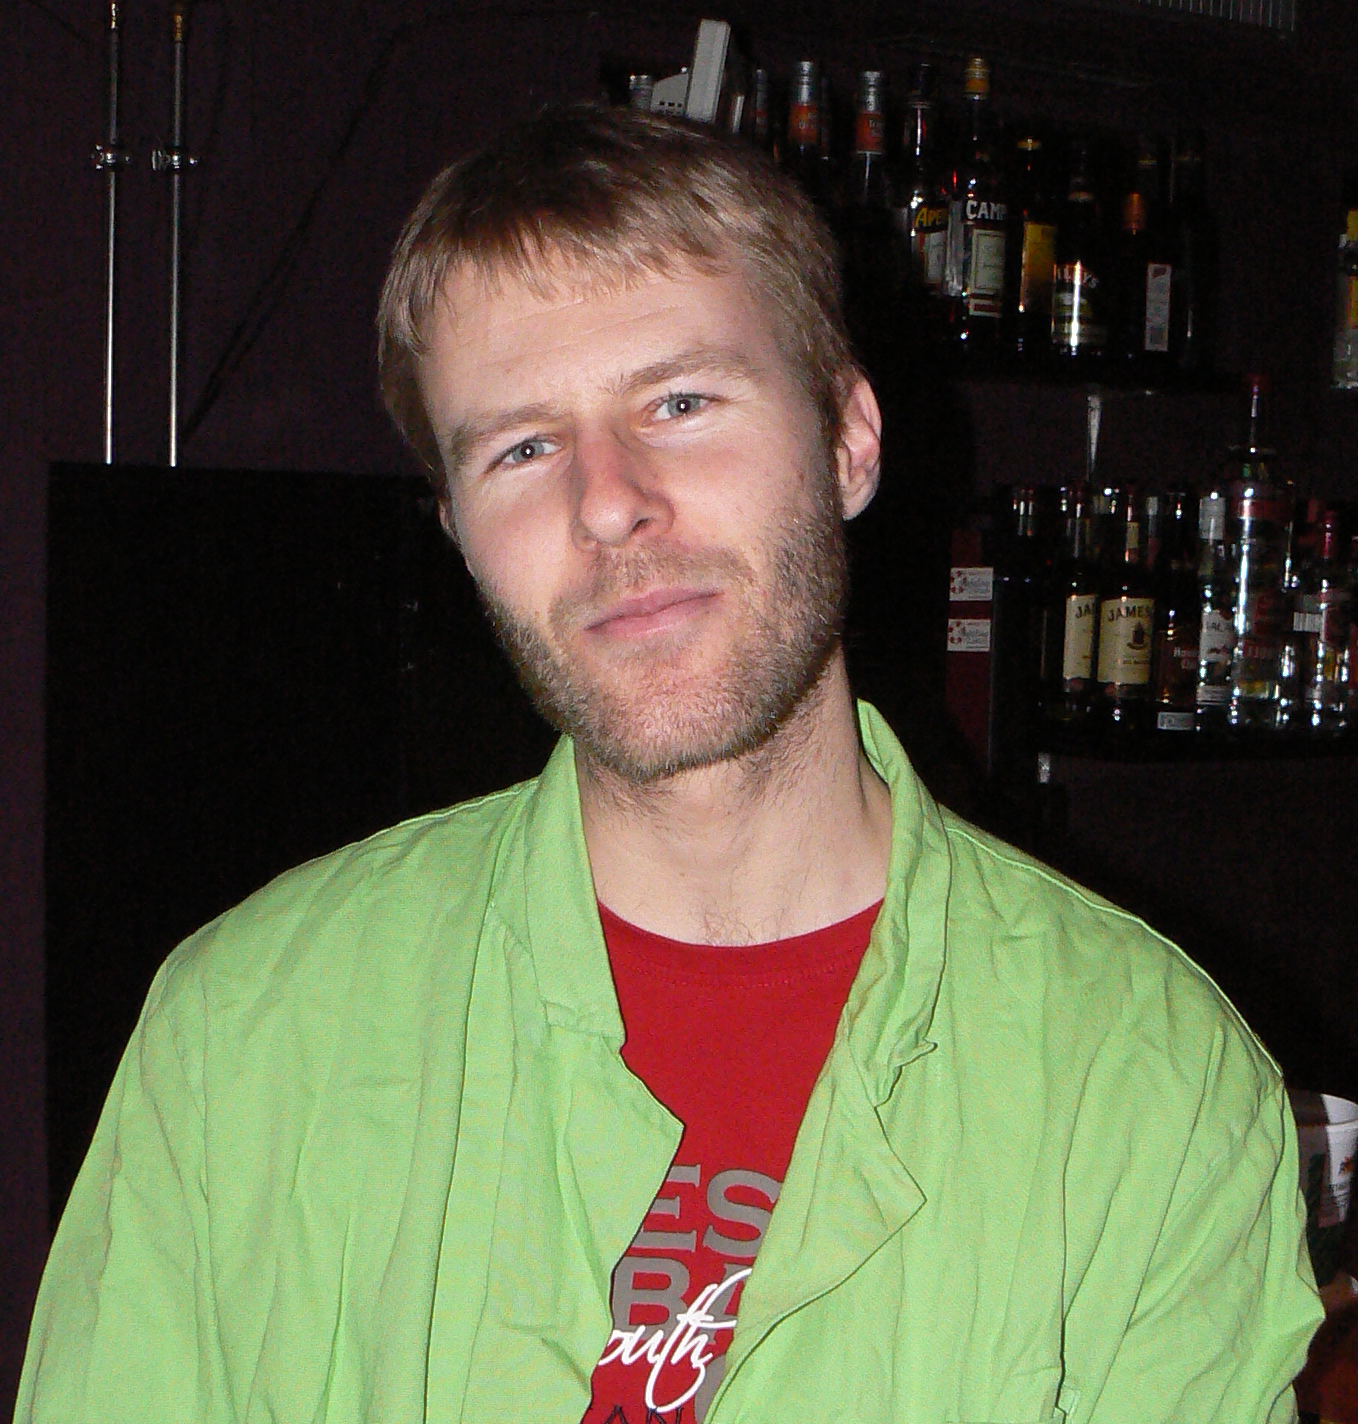
\includegraphics[width = 0.2 \textwidth]{Figures/Pirmin}};
				\node (judith) at ($(pirmin)+(1.2,0)$) {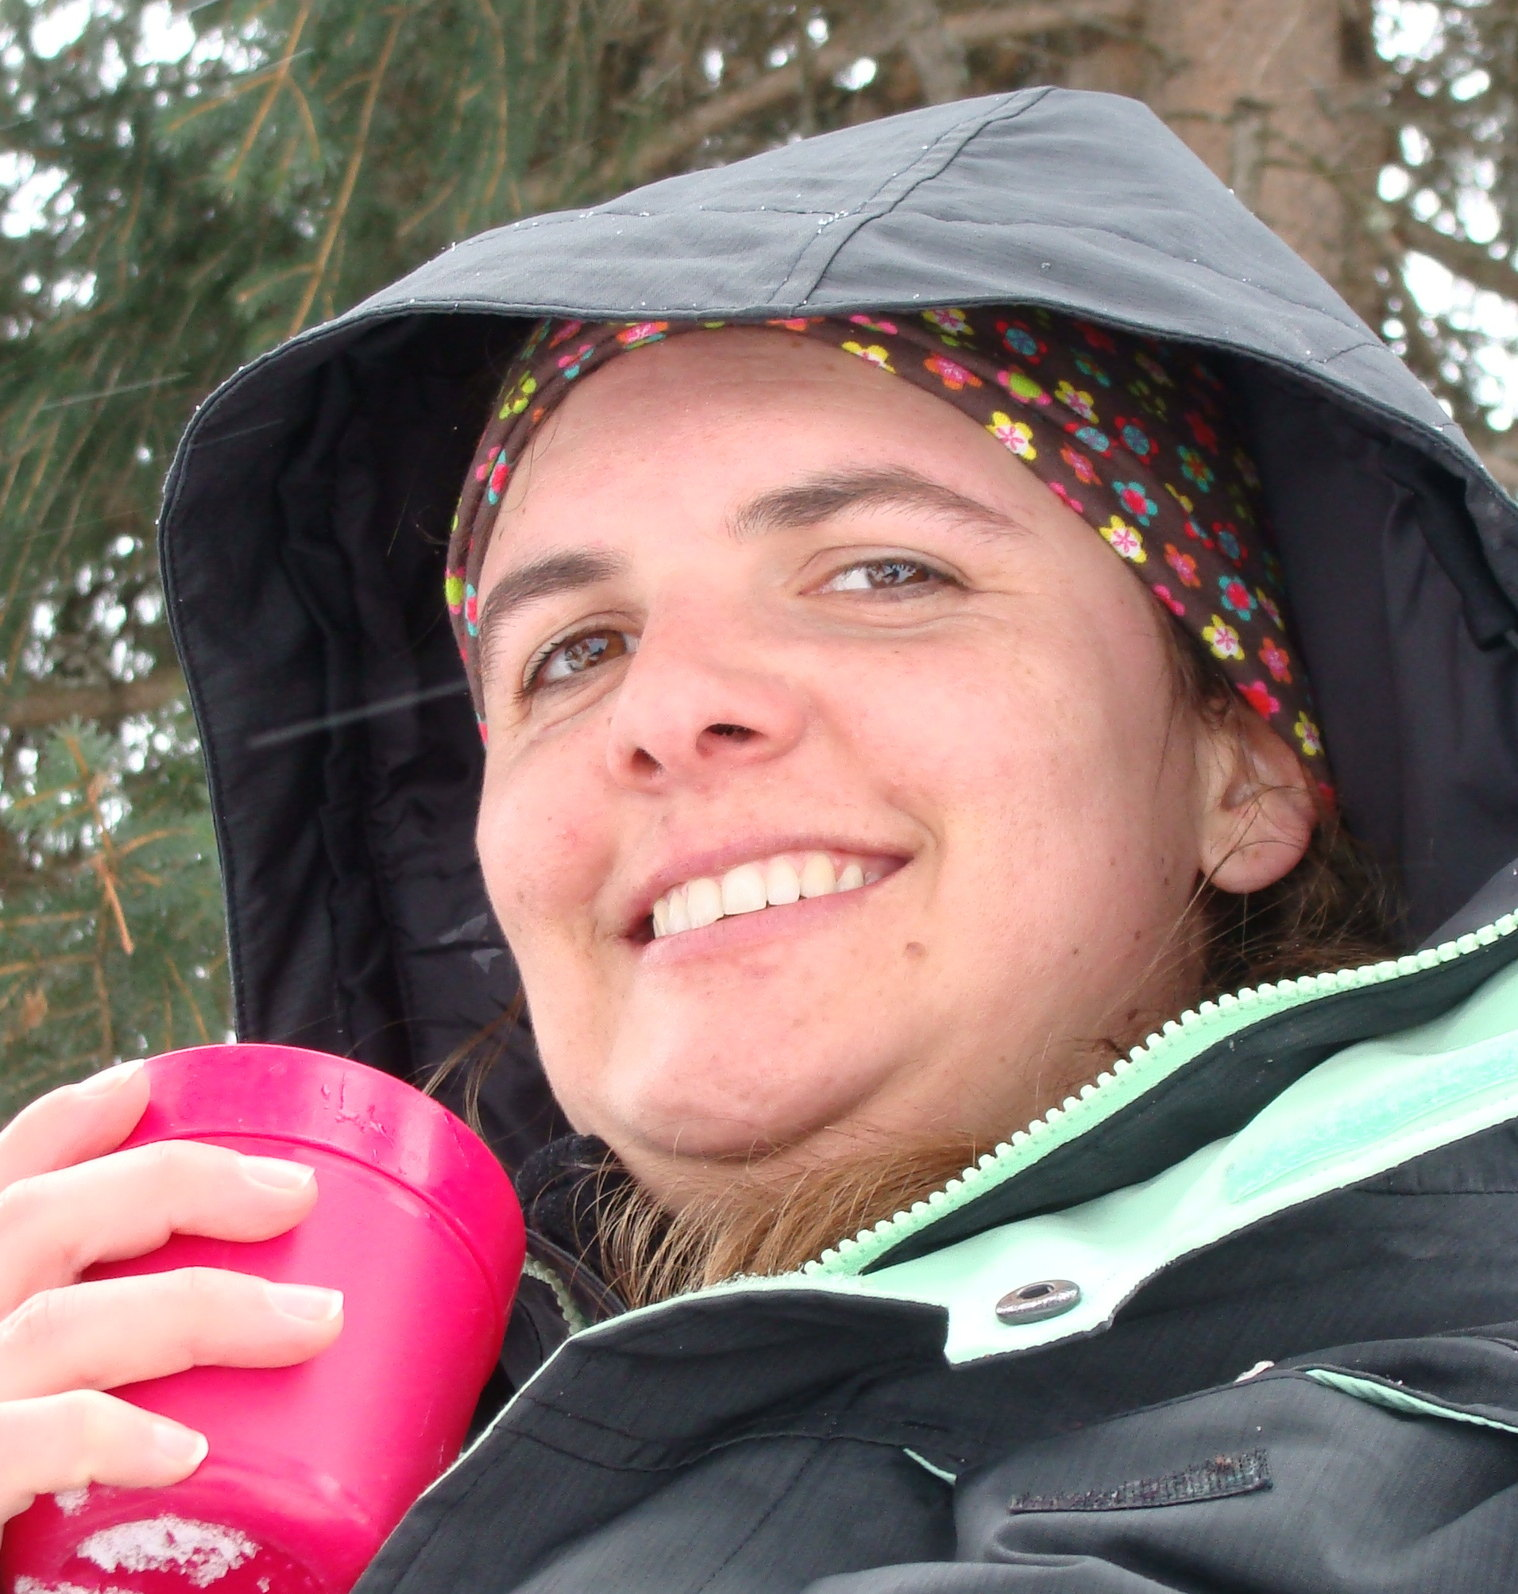
\includegraphics[width = 0.18 \textwidth]{Figures/Judith}};
				
				\node (nina) at ($(koen)+(0,-1.4)$) {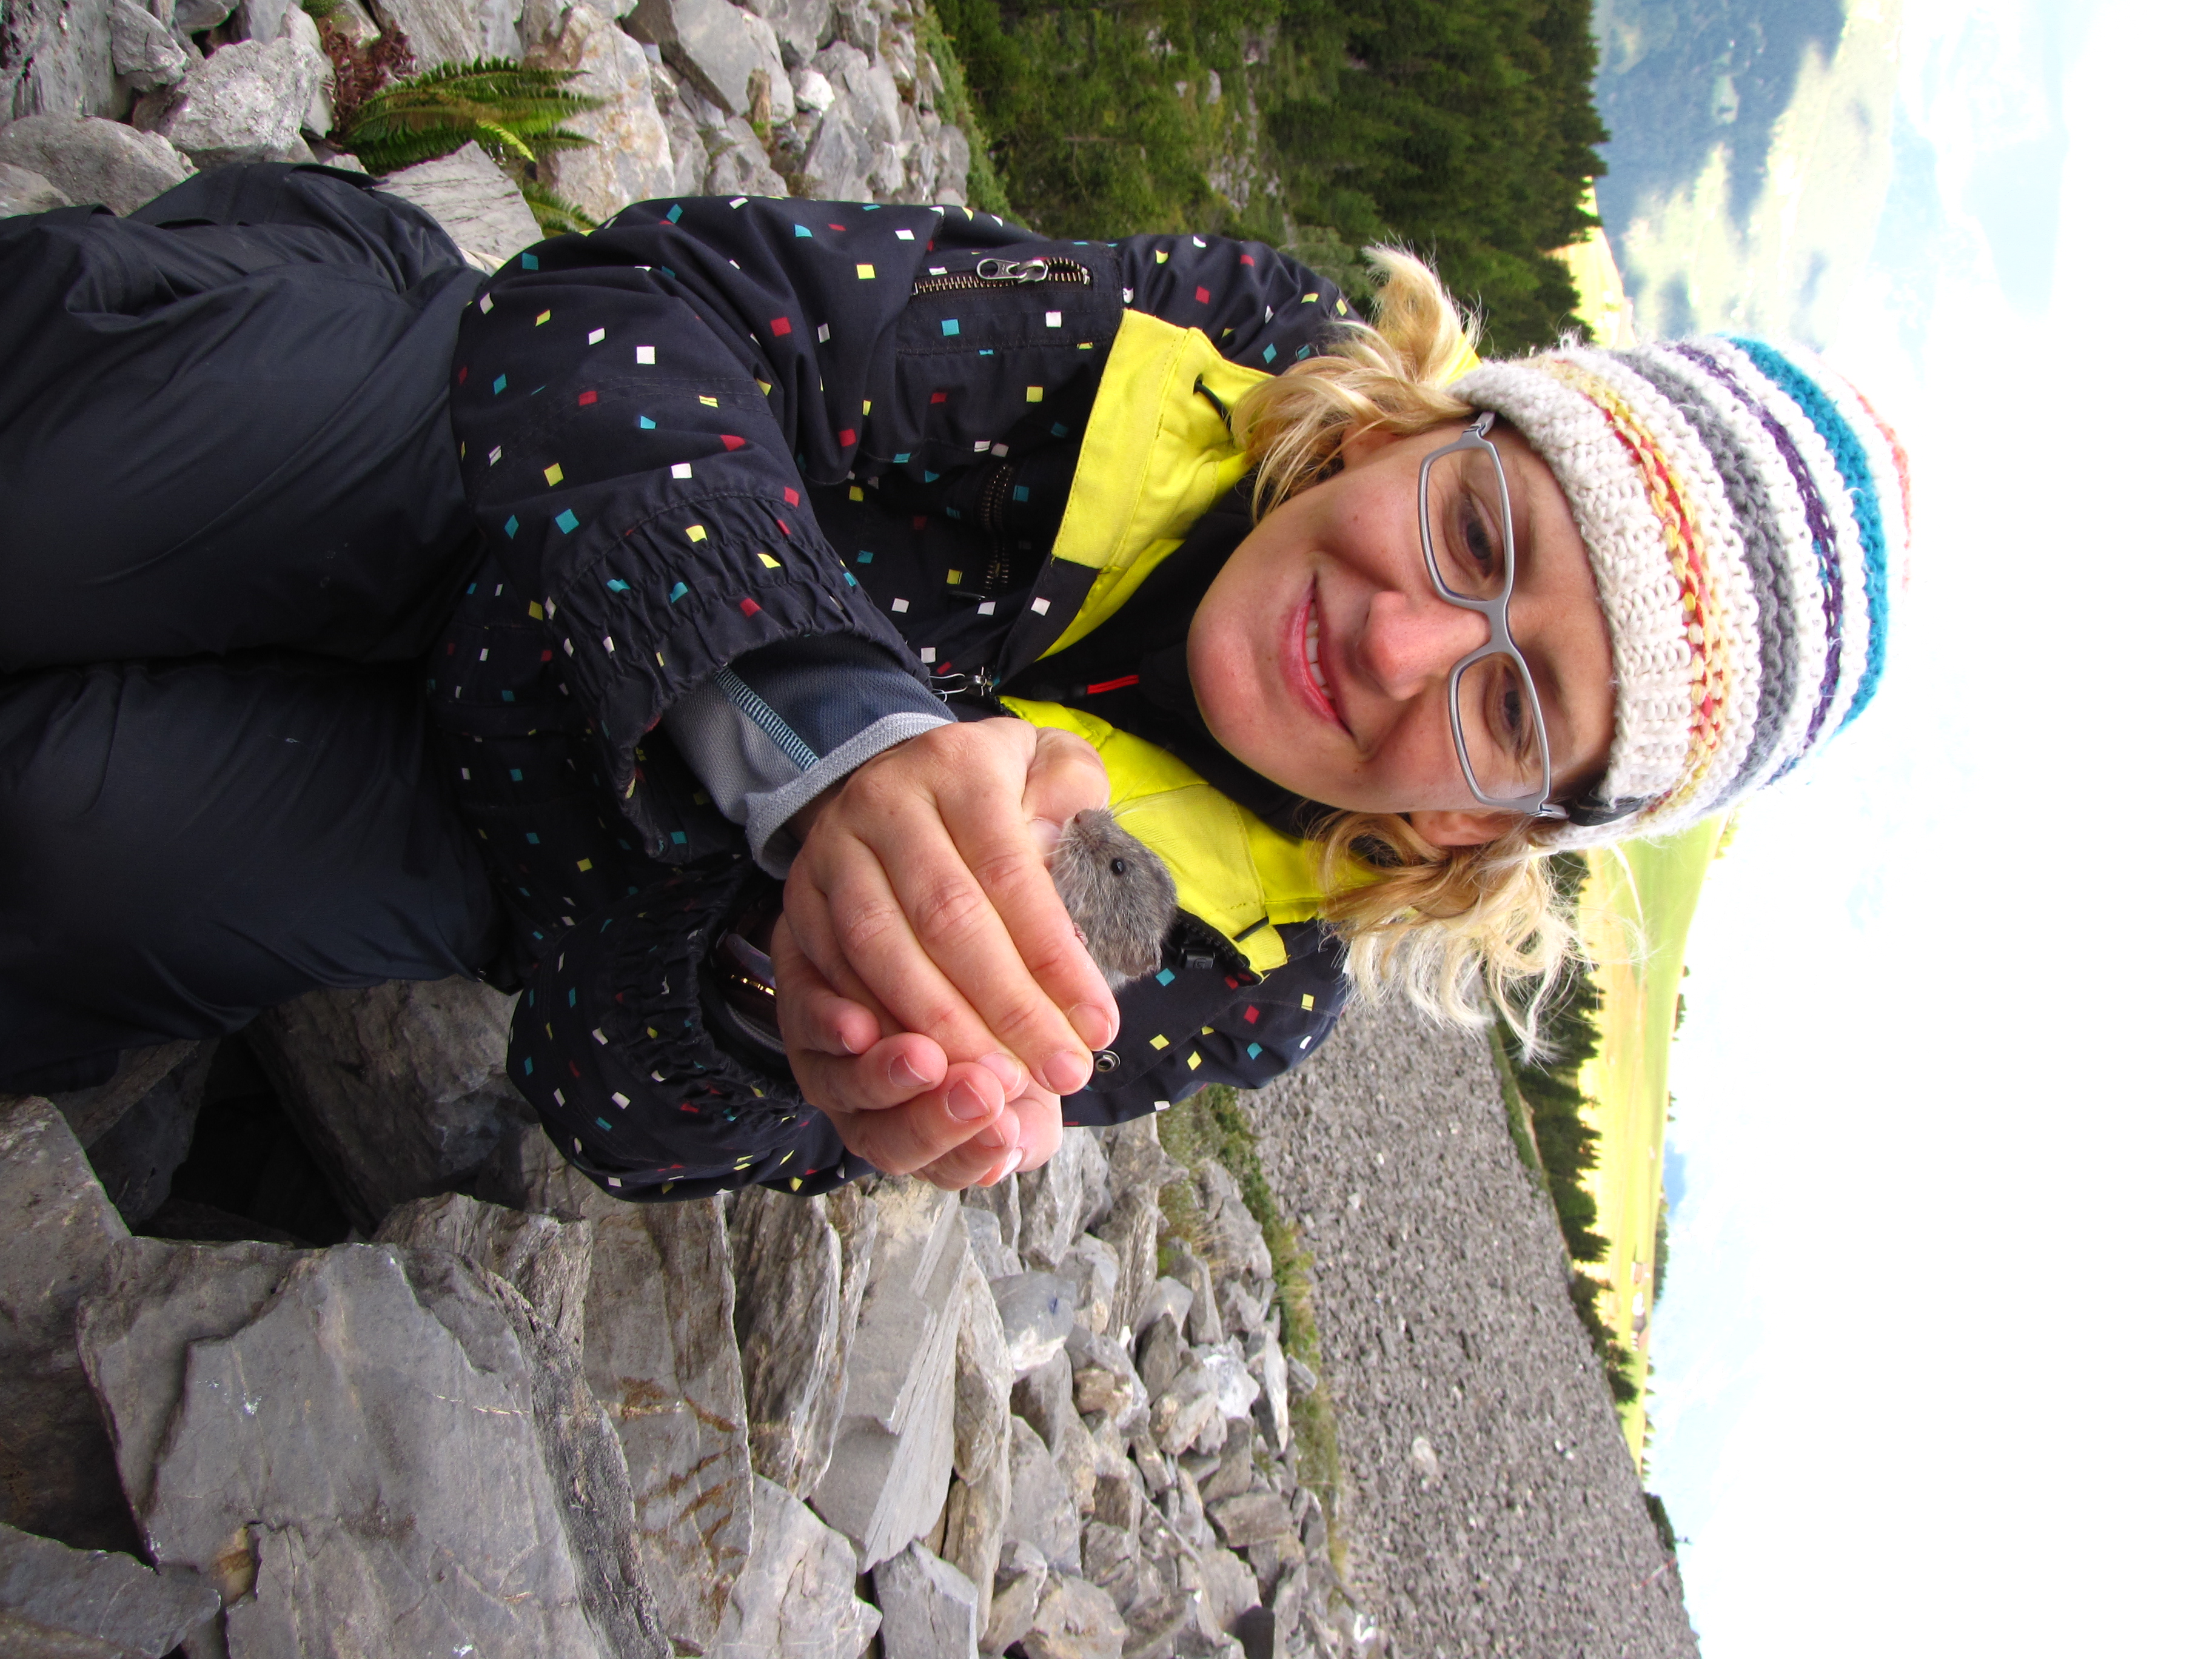
\includegraphics[width = 0.2 \textwidth]{Figures/Nina}};
				\node (hedwig) at ($(nina)+(1.2,0)$) {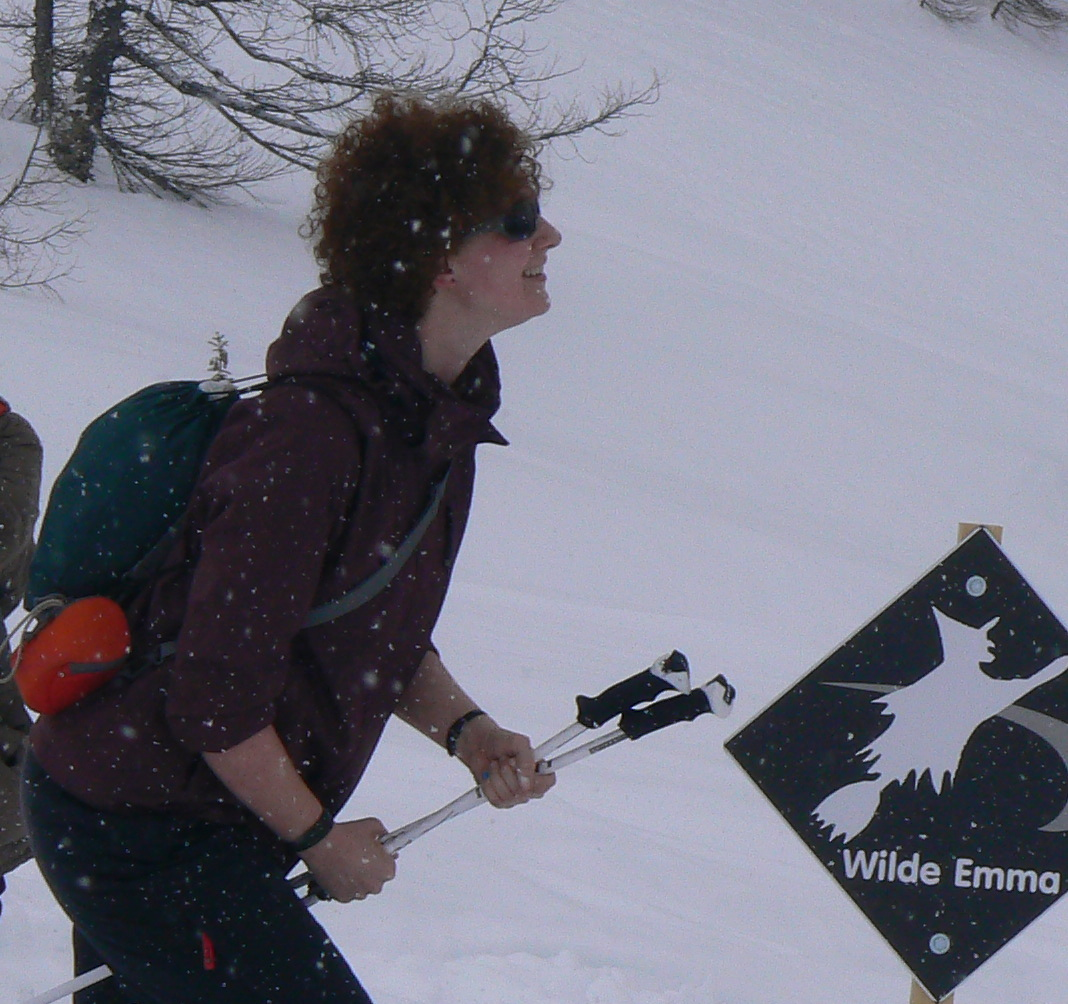
\includegraphics[width = 0.2 \textwidth]{Figures/Hedwig}};
				\node (kasia) at ($(hedwig)+(1.2,0)$) {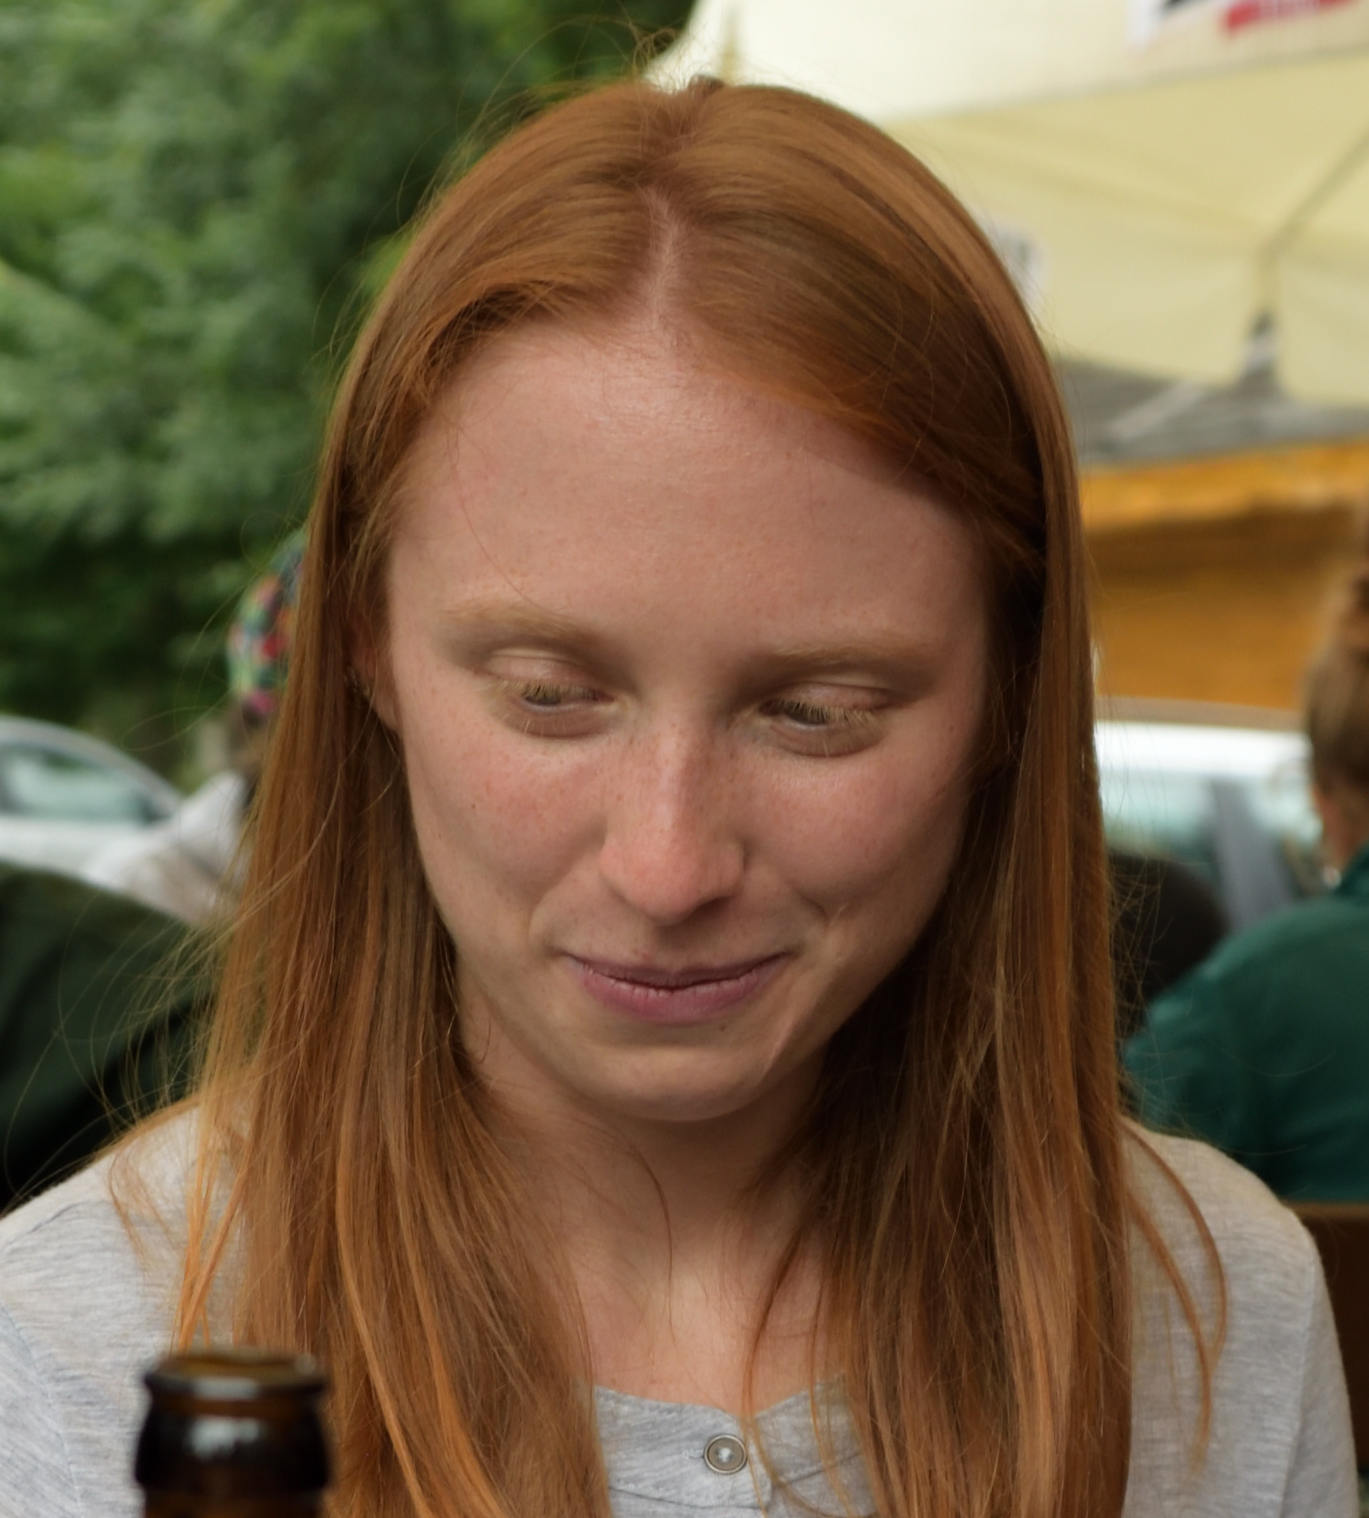
\includegraphics[width = 0.2 \textwidth]{Figures/Kasia}};
				\node (simon) at ($(kasia)+(1.2,0)$) {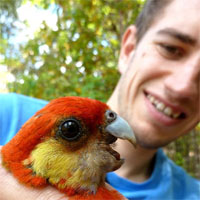
\includegraphics[width = 0.15 \textwidth]{Figures/Simon}};
				\node (chelsea) at ($(simon)+(1.3,0)$) {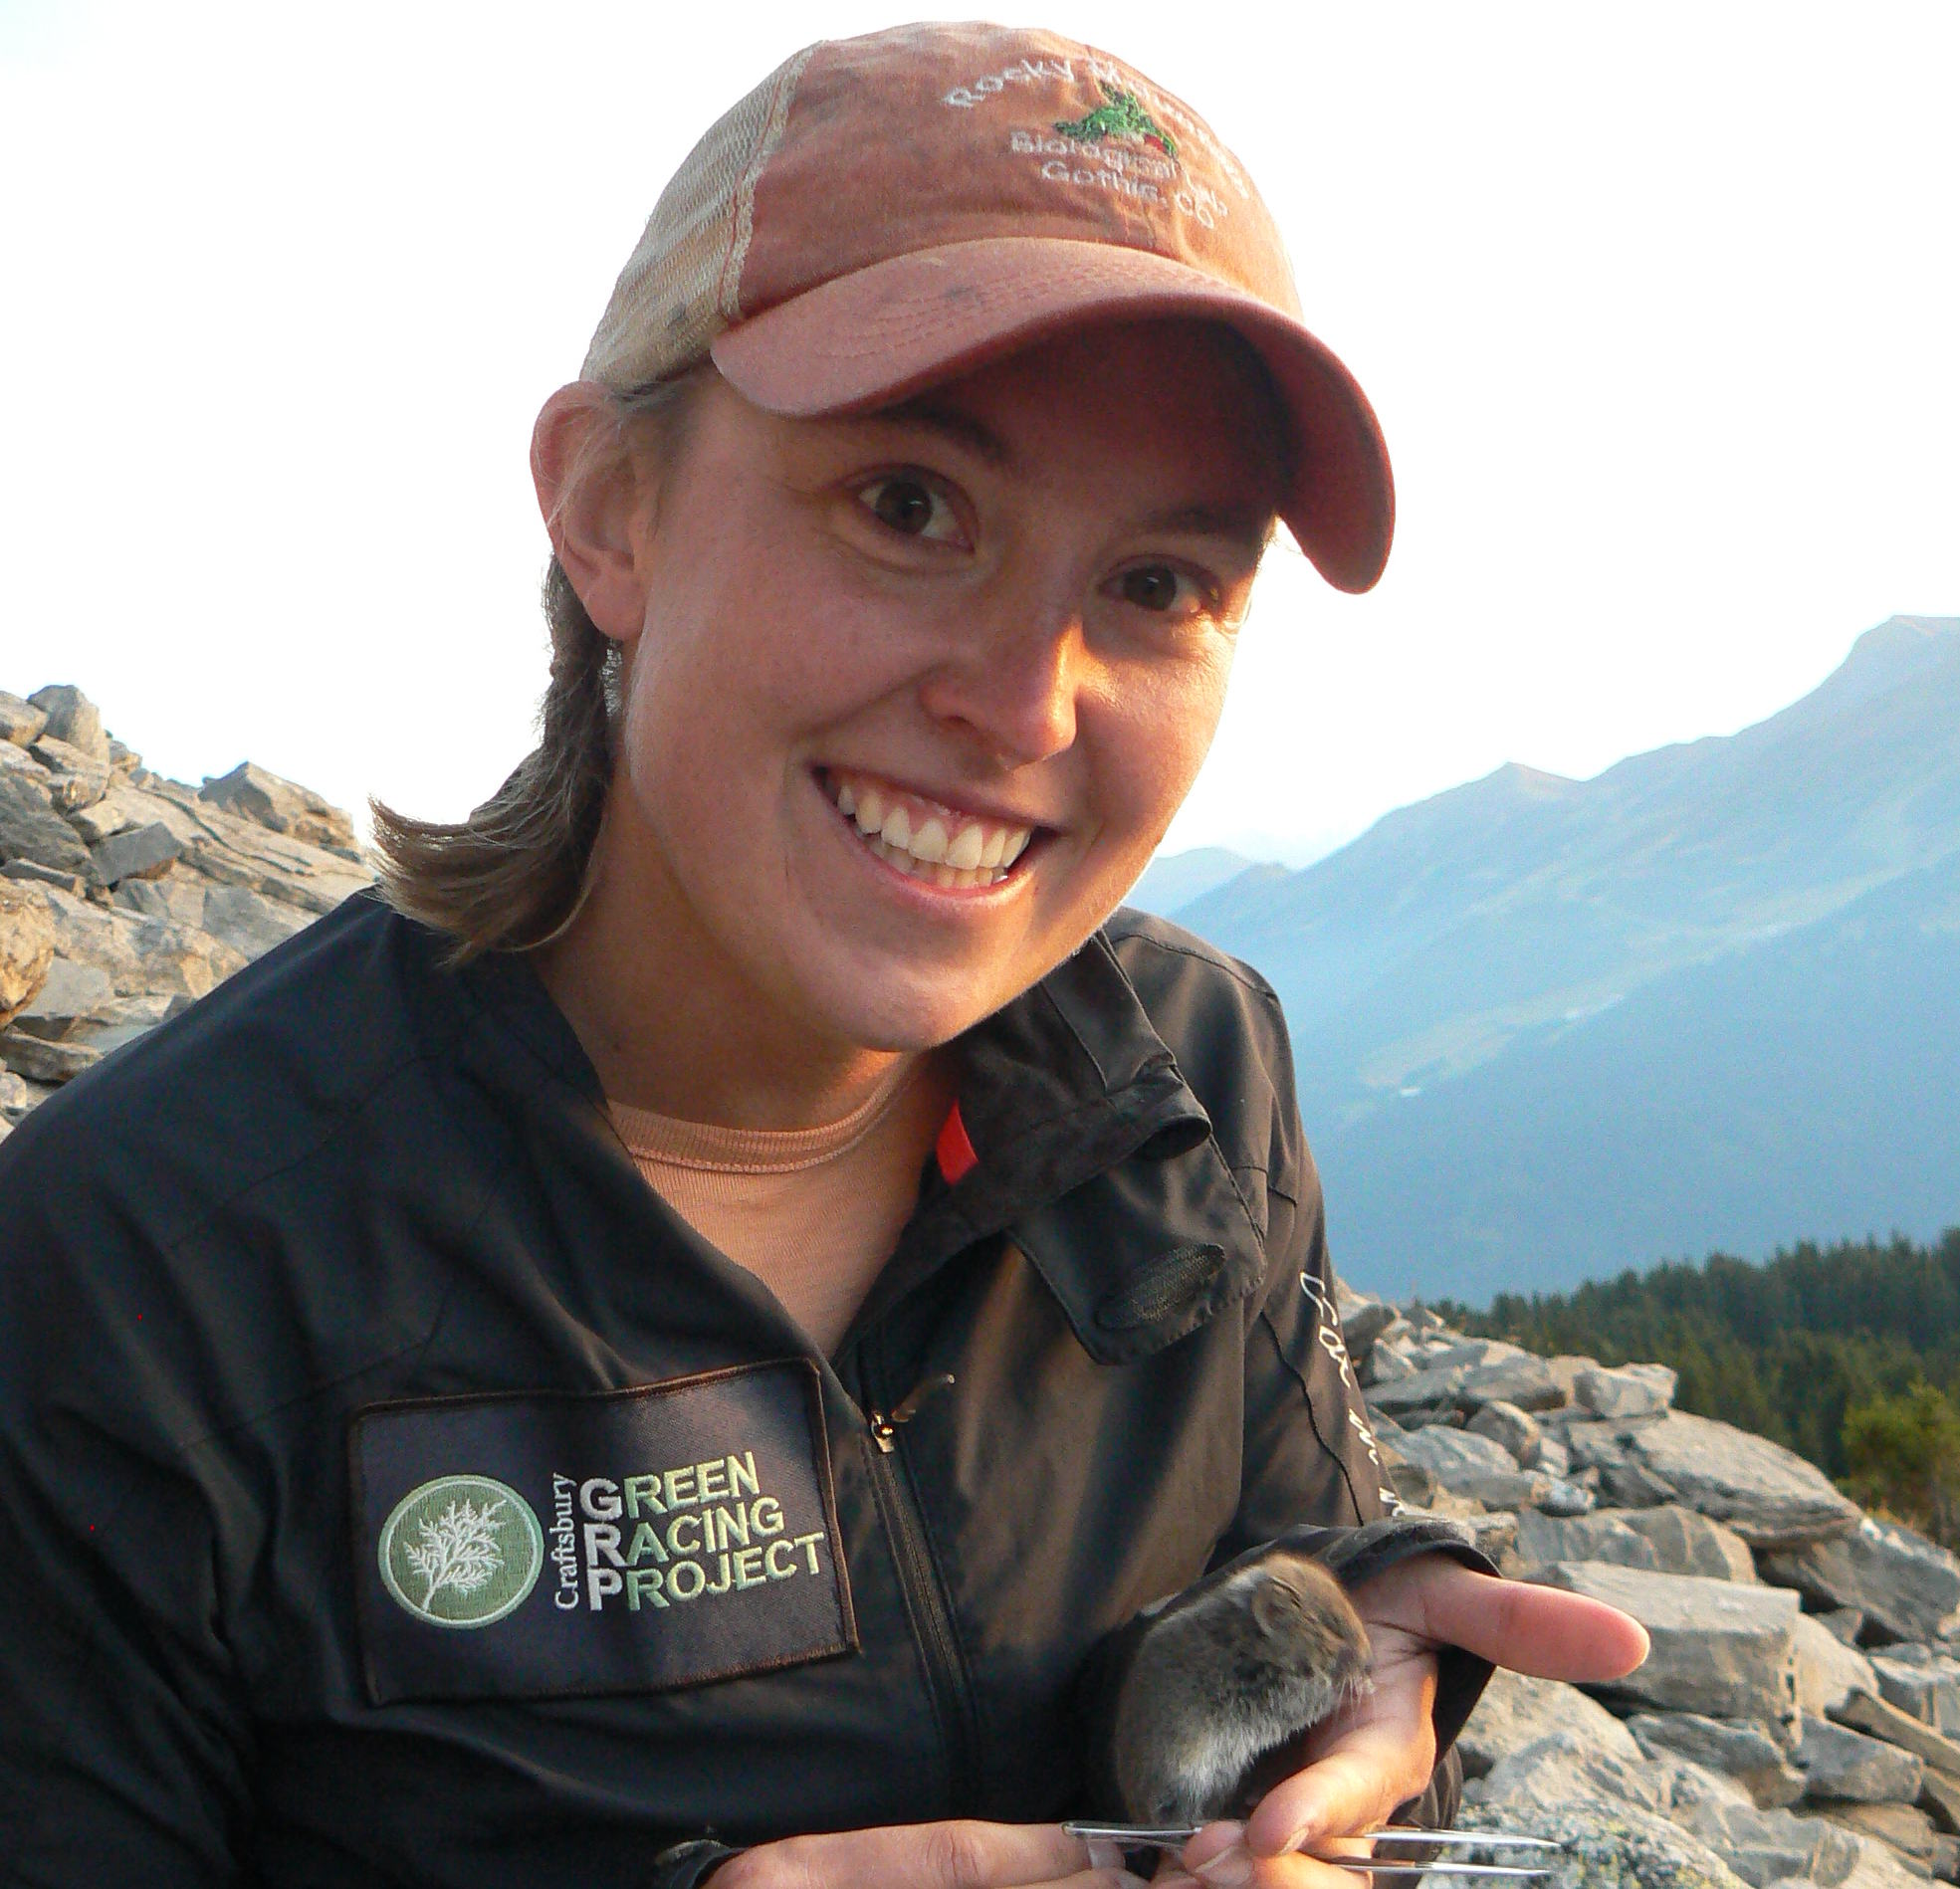
\includegraphics[width = 0.2 \textwidth]{Figures/Chelsea}};
				\node (ashley) at ($(chelsea)+(1.2,0)$) {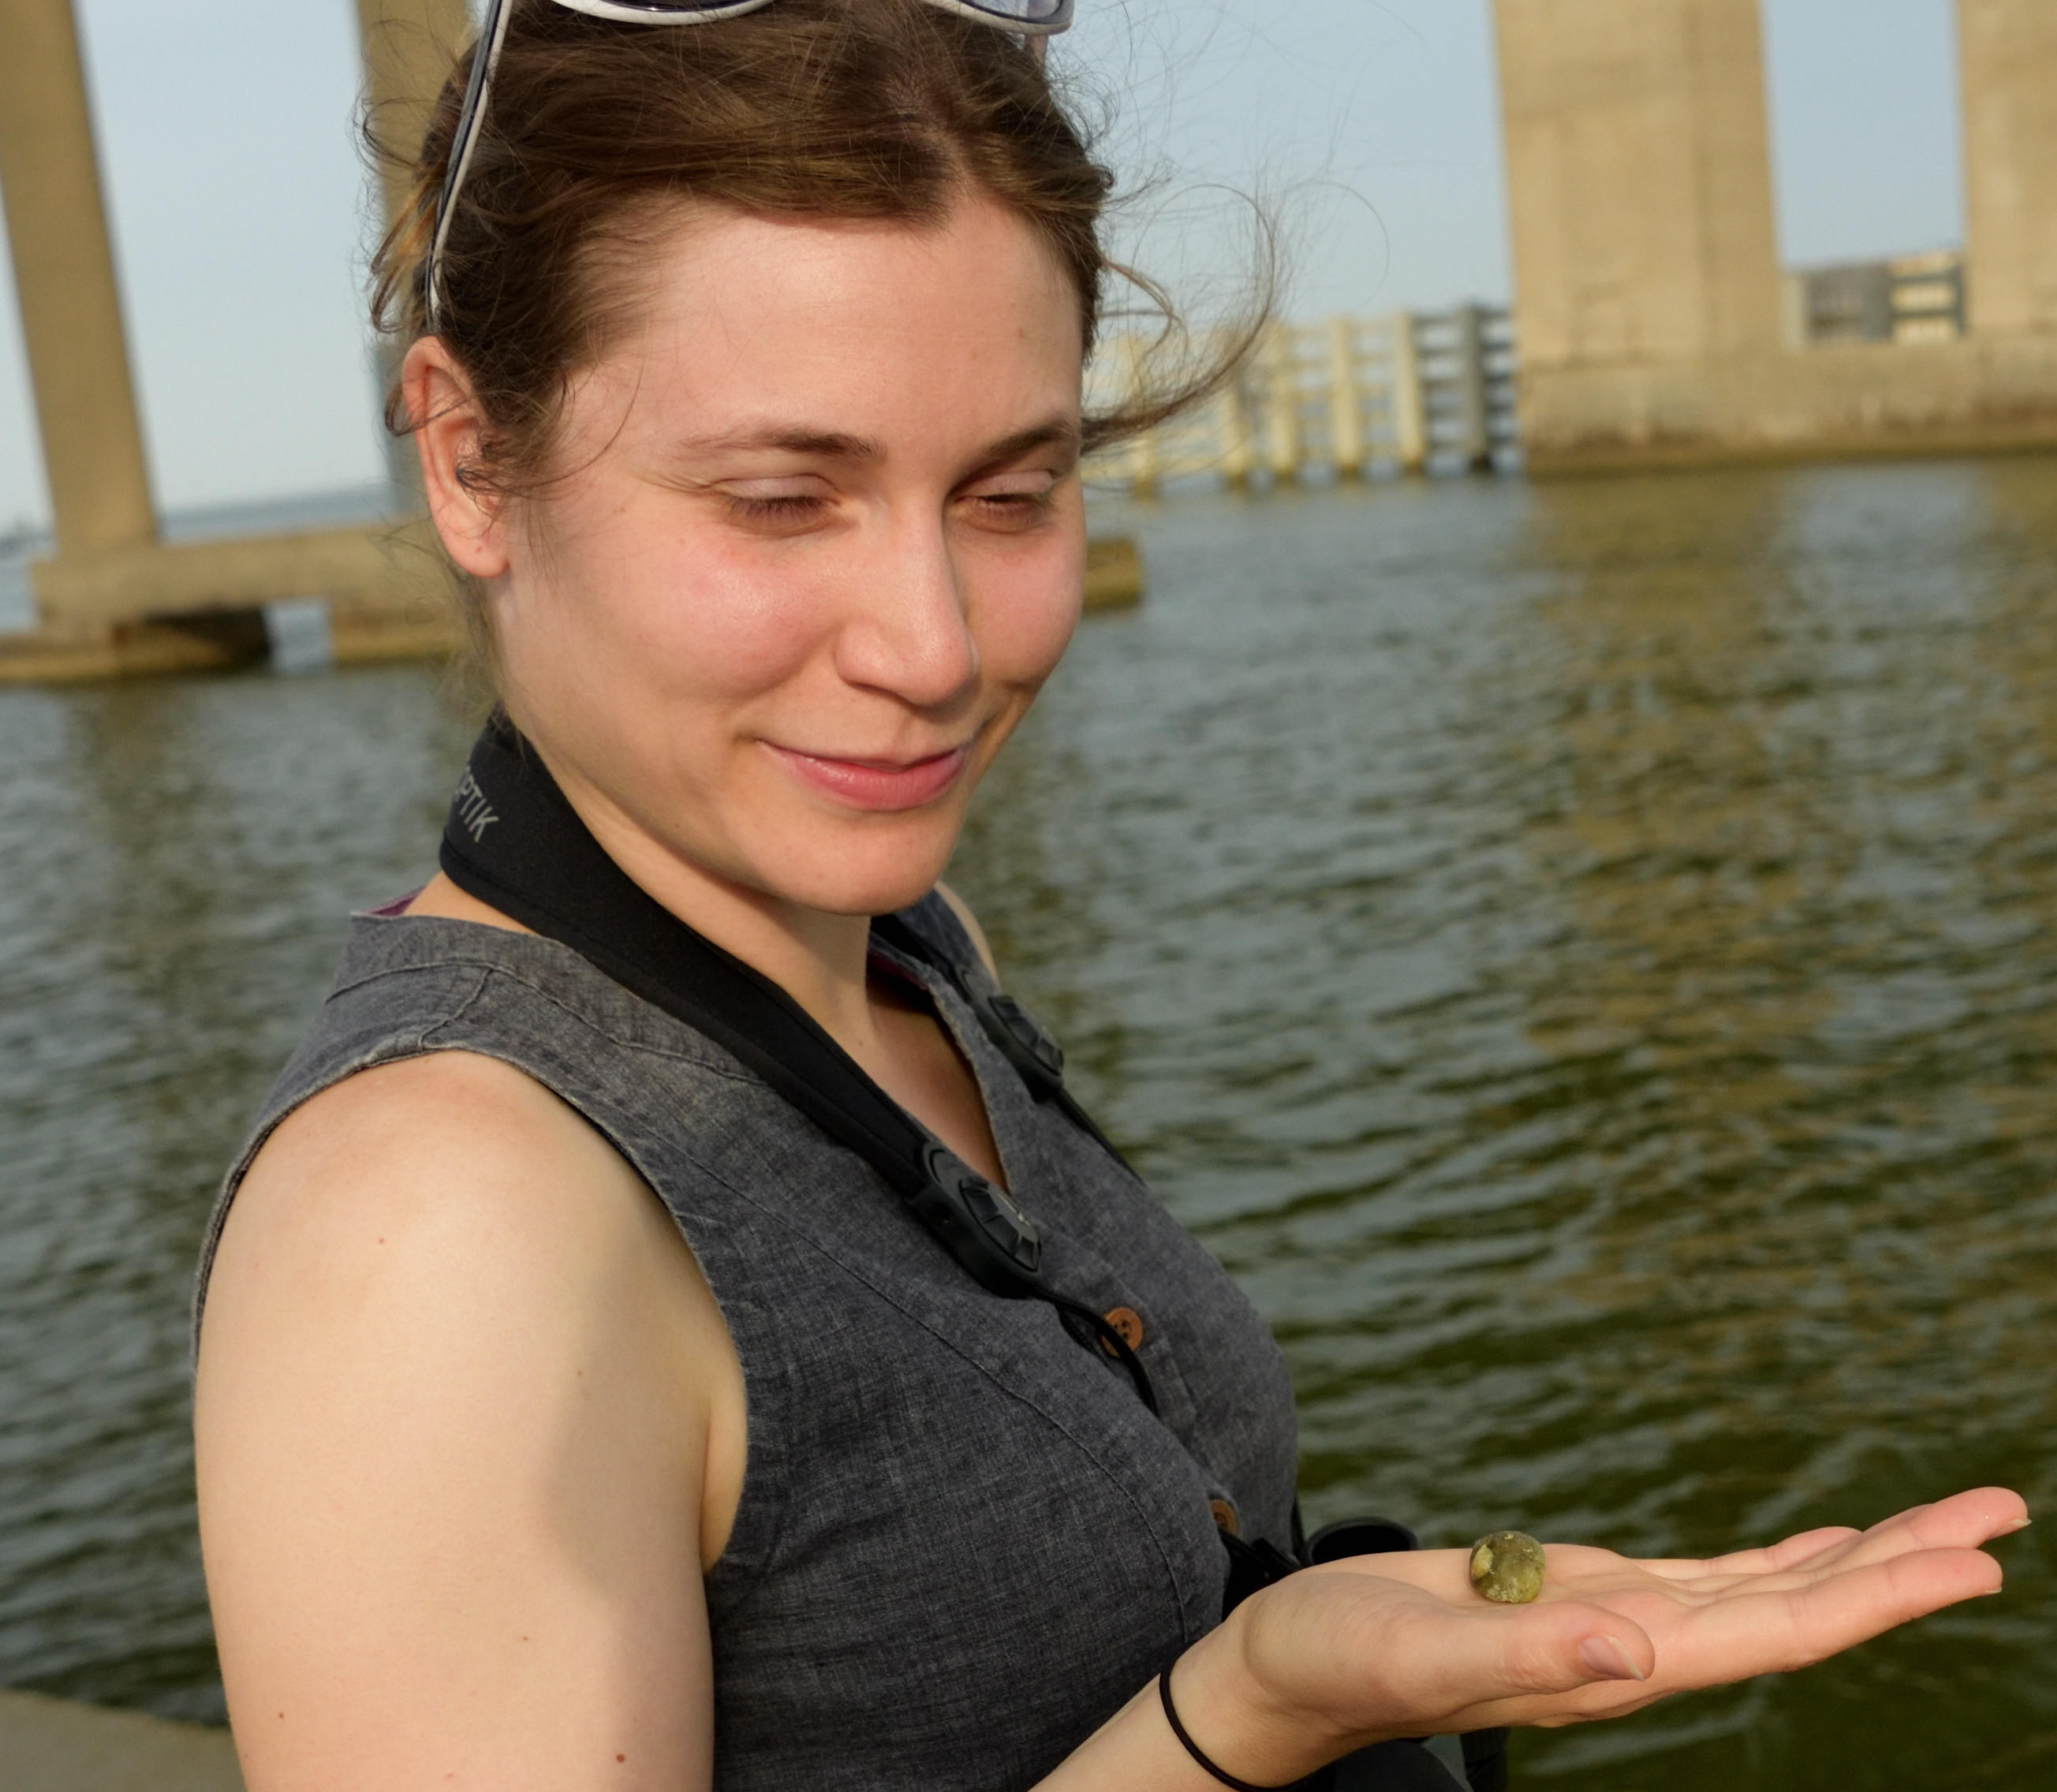
\includegraphics[width = 0.2 \textwidth]{Figures/Ashley}};

%%%%%%		
				\node (beni) at ($(nina)+(0,-1.4)$) {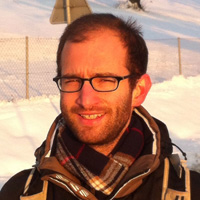
\includegraphics[width = 0.2 \textwidth]{Figures/Beni}};
				\node (alex) at ($(beni)+(1.2,0)$) {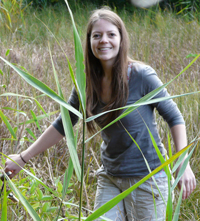
\includegraphics[width = 0.2 \textwidth]{Figures/Alex}};
				\node (rassim) at ($(alex)+(1.2,0)$) {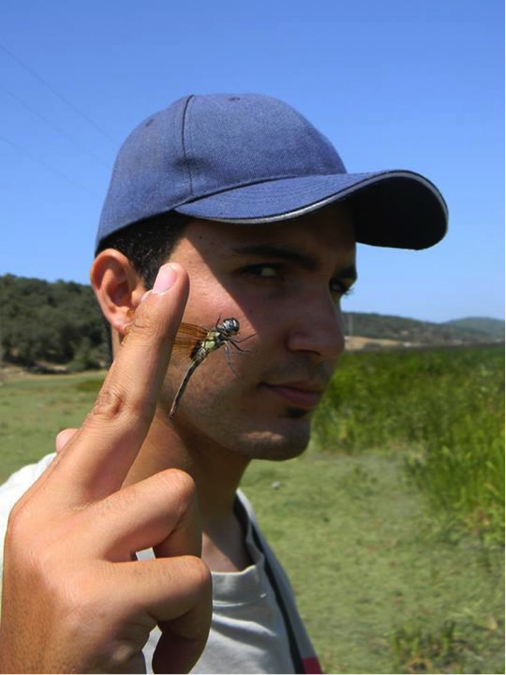
\includegraphics[width = 0.2 \textwidth]{Figures/Rassim}};
				\node (debbie) at ($(rassim)+(1.2,0)$) {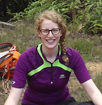
\includegraphics[width = 0.2 \textwidth]{Figures/Debbie}};
				\node (gianalberto) at ($(debbie)+(1.2,0)$) {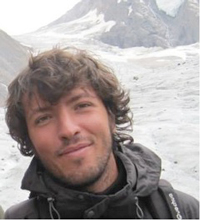
\includegraphics[width = 0.2 \textwidth]{Figures/Gianalberto}};
				\node (peter) at ($(gianalberto) +(1.2,0)$) {\includegraphics[width = 0.2 \textwidth]{Figures/Peter}};
				%%%%
				\node (jelena) at ($(beni)+(0,-1.4)$) {\includegraphics[width = 0.2 \textwidth]{Figures/Jelena}};
				\node (hanna) at ($(jelena)+(1.2,0)$) {\includegraphics[width = 0.2 \textwidth]{Figures/Hanna}};
				\node (jasmin) at ($(hanna)+(1.2,0)$) {\includegraphics[width = 0.2 \textwidth]{Figures/Jasmin}};
				\node (josh) at ($(jasmin)+(1.2,0)$)  {\includegraphics[width = 0.2 \textwidth]{Figures/Josh}};
				\node (wolf) at ($(josh)+(1.2,0)$) {\includegraphics[width = 0.2 \textwidth]{Figures/Wolf}};
				\node (bea) at ($(koen)+(0,-1.4)$) {\includegraphics[width = 0.2 \textwidth]{Figures/Bea}};
				\node (ninag) at ($(koen)+(0,-1.4)$) {\includegraphics[width = 0.2 \textwidth]{Figures/NinaG}};
				\node (anais) at ($(koen)+(0,-1.4)$) {\includegraphics[width = 0.2 \textwidth]{Figures/Anais}};
				\node (isobel) at ($(koen)+(0,-1.4)$) {\includegraphics[width = 0.2 \textwidth]{Figures/Isobel}};
				\node (erika) at ($(koen)+(0,-1.4)$) {\includegraphics[width = 0.2 \textwidth]{Figures/Erika}};
				\node (rien) at ($(koen)+(0,-1.4)$) {\includegraphics[width = 0.2 \textwidth]{Figures/Rien}};
				\node (vanja) at ($(koen)+(0,-1.4)$) {\includegraphics[width = 0.2 \textwidth]{Figures/Vanja}};
				
				\node (christine) at ($(koen)+(0,-1.4)$) {\includegraphics[width = 0.2 \textwidth]{Figures/Christine}};
				
				
			\end{tikzpicture}
		\end{figure}
	\end{column}
	\end{columns}
\end{frame}
%%%%%%%%%%%
%Intro on variation within species/population
%Explain causes of variation imply consequences

\begin{frame}{Phenotypic variation within population}
	\begin{figure}
		\includegraphics[width = 0.6 \textwidth]{Figures/Humansize}
	\end{figure}
	\begin{figure}
		\includegraphics[width = 0.45 \textwidth]{Figures/Cepaea}\hspace{0.1cm}		
		\includegraphics[width = 0.45 \textwidth]{Figures/Harmonia}
	\end{figure}
\end{frame}
%%%%%%%%%%%

\begin{frame}
	\begin{figure}
		\includegraphics[width=0.4\textwidth,height=0.3\textwidth]{Figures/babyTurtle} \hspace{1pt}
		\includegraphics[width=0.4\textwidth,height=0.3\textwidth]{Figures/adultTurtle}
		\vspace{1pt}
		\includegraphics[width=0.4\textwidth,height=0.3\textwidth]{Figures/BlueTits2}\hspace{1pt}
		\includegraphics[width=0.4\textwidth,height=0.3\textwidth]{Figures/BlueTits8}
	\end{figure}
\end{frame}

%%%%%%%%%%%%%%%%%%%%%%%%%%%%%%%%%%%%%%%%%%%%%%%%%%%%%%
%%%%%%%%%%%%%%%%%%%%%%% Chap 1 %%%%%%%%%%%%%%%%%%%%%%%
%%%%%%%%%%%%%%%%%%%%%%%%%%%%%%%%%%%%%%%%%%%%%%%%%%%%%%
%Dice!
\begin{frame}

\end{frame}

%%%%%%%%%%%%%%%%%%%%%%%%%%%%%%%%%%%%%%%%%%%%%%%%%%%%%%
%%%%%%%%%%%%%%%%%%%%%%% Chap 2 %%%%%%%%%%%%%%%%%%%%%%%
%%%%%%%%%%%%%%%%%%%%%%%%%%%%%%%%%%%%%%%%%%%%%%%%%%%%%%



%FIeld and population
\begin{frame}[plain]{}
	\begin{figure}
	\centering
		\includegraphics[height= \textheight]{Figures/SnowBall}
	\end{figure}
\end{frame}
%%%%%%%%%%%

\begin{frame}{Snow vole (\textit{Chionomys nivalis}, Martins 1842)}

\begin{columns}
	\begin{column}[c]{0.5\textwidth}
		\begin{itemize}[<+->]
			\item NOT white
			\item Rock-dweller
			\item 30-45g
			\item 10-14cm long $+$ 5-8cm tail
			\item Slow life pace
		\end{itemize}
	\end{column}
	\begin{column}[c]{0.5\textwidth}
	\begin{figure}
	\centering
		\includegraphics[width= \textwidth]{Figures/P1250035}
	\end{figure}
	\end{column}
	\end{columns}
\end{frame}
%%%%%%%%%%%



\begin{frame}[plain]{}
	\begin{figure}
	\centering
		\includegraphics[height= \textheight]{Figures/map-1}
	\end{figure}
\end{frame}
%%%%%%%%%%%

\begin{frame}[plain]{}
	\begin{figure}
	\centering
		\begin{tikzpicture}
			
			\node (pic) at (0,0) {\includegraphics[width= 0.95\textwidth]{Figures/DSC_2111viewontaliflue}};
			\draw[rounded corners,thick,color=red] (-1.2,-0.8) rectangle (0.5,0);
		\end{tikzpicture}
	\end{figure}
\end{frame}
%%%%%%%%%%%

\begin{frame}[plain]{}
	\begin{figure}
	\centering
		\includegraphics[width= \textwidth]{Figures/fieldposts2}
	\end{figure}
\end{frame}
%%%%%%%%%%%

\begin{frame}[plain]{}
	\begin{figure}
	\centering
		\includegraphics[width= \textwidth]{Figures/boulder}
	\end{figure}
\end{frame}
%%%%%%%%%%%

\begin{frame}[plain]{}
	\begin{figure}
	\centering
		\includegraphics[width= \textwidth]{Figures/DSC_2027trap}
	\end{figure}
\end{frame}
%%%%%%%%%%%

\begin{frame}{What we measure}

\begin{columns}
	\begin{column}[c]{0.4\textwidth}
		\begin{itemize}
			\item<2-> Morphology
				\begin{itemize}
					\item Body mass 
					\item Body length
					\item Tail length
				\end{itemize}
			\item<3-> Capture/Recaptures
				\begin{itemize}
					\item Death/emigration
					\item Location
				\end{itemize}
			\item<4-> DNA
				\begin{itemize}
					\item 20 ``neutral'' markers
					\item Sex identification
					\item Any genotyping
					\item<5-> \textbf{Pedigree}
				\end{itemize}
		\end{itemize}
	\end{column}
	
	\begin{column}[c]{0.6\textwidth}

	\centering
		\only<2>{\includegraphics[height= \textheight]{Figures/CN2015_MeulenbroekLiz_00024}}
		\only<3>{\includegraphics[height= \textheight]{Figures/CN2015_MeulenbroekLiz_00022}}
		\only<4>{\includegraphics[height= \textheight]{Figures/IMG_20160916_075241}}
		\only<5>{\includegraphics[height= 0.5\textheight]{Figures/familytree}}
		\only<6>{\includegraphics[height= \textheight]{Figures/pedigreeplot}}

	\end{column}
\end{columns}
\end{frame}
%%%%%%%%%%%


%%%%%%%%%%%%%%%%%%%%%%%%%%%%%%%%%%%%%%%%%%%%%%%%%%%%%%
%%%%%%%%%%%%%%%%%%%%%%% Chap 3 %%%%%%%%%%%%%%%%%%%%%%%
%%%%%%%%%%%%%%%%%%%%%%%%%%%%%%%%%%%%%%%%%%%%%%%%%%%%%%

%Open some dice! -> DNA and grass in it, leading to most common number...

%%%%%%%%%%%%%%%%%%%%%%%%%%%%%%%%%%%%%%%%%%%%%%%%%%%%%%
%%%%%%%%%%%%%%%%%%%%%%% Chap 4 %%%%%%%%%%%%%%%%%%%%%%%
%%%%%%%%%%%%%%%%%%%%%%%%%%%%%%%%%%%%%%%%%%%%%%%%%%%%%%



\end{document}
